\chapter{基于程序性质图的源代码软件漏洞挖掘方法研究}

根据Rice定理\upcite{rice_classes_1953},通过一个程序完全的自动检测其他程序的复杂属性是不可行的。
一般的源代码静态分析工具都是基于字符串匹配或者抽象语法树匹配的,
所以现行的工具要么局限于特定类型的漏洞,要么需要大量的人工审计工作\upcite{heelan_vulnerability_2011}消除误报。例如PREfast\upcite{bush_static_2000}、RATS\upcite{wnoauthor_cern_nodate}以及PScan\upcite{dekok_pscan:_2000}虽然能够检测一些程序开发过程中产生的漏洞,但是很难检测成因复杂的漏洞。而另外一些工具,例如Splint\upcite{noauthor_splint_nodate}只能检测特定的漏洞。

%审计像Linux内核这样具有庞大代码量的软件系统是一件不可能完成的事情。基于动态测试的方法,例如模糊测试和符号执行,虽然能够挖掘不同类型的漏洞而且能够产生测试用例,但是符号执行随着软件规模的增加会出现路径爆炸问题,此外符号执行还有交互环境模拟问题以及约束求解器求解能力的限制问题;模糊测试则存在随机性强,代码覆盖率低的问题。所以,首先漏进行洞可疑区域标定然后再动态测试可疑区域是一个解决办法。

针对C/C++源代码软件,本章提出了一种基于程序性质图的源代码漏洞挖掘方法。该方法利用程序性质图聚合抽象语法树、控制流图、数据流图三种中间表示,通过定义以及组合不同的程序性质图遍历方式能够检测多种源代码软件漏洞。
%对于缓冲区溢出漏洞,影响漏洞的特征有很多种,漏洞的形成是多个特征综合作用的结果。
针对缓冲区溢出漏洞挖掘精确度不高的问题,
本章提出了一种基于机器学习的缓冲区溢出漏洞挖掘方法。该方法首先将缓冲区溢出静态特征分成7类;然后,在已标记的漏洞中,利用扩展的程序性质图获取静态特征并将其映射到向量空间,作为机器学习算法的训练集;最后,选取5种有监督机器学习算法在训练集中训练分类器,并通过分类器在新的源代码中挖掘缓冲区溢出漏洞。

\section{程序性质图生成}\label{程序性质图生成}

程序性质图(Code Property Graph,CPG)是源代码在性质图(Property Graph,PG)\upcite{rodriguez_graph_2010}上的表现形式。本节介绍了性质图的概念、各种中间表示的生成过程、程序性质图以及程序性质图的各种遍历方式。

\subsection{性质图}

在图理论当中,有向图可以用一个关系对表示,$G=(V,E)$,$V$是节点集合,$E\subseteq(V \times V)$是节点之间边的集合。性质图的节点具有以下特性:{(1)}每个节点都对应一个唯一标识符;{(2)}每个节点都包含一个入边和出边集;{(3)}每个节点都包含键-值集。性质图的边具有相似的性质:{(1)}每条边对应一个唯一标识符;{(2)}每条边都包含一个标签表示边的类型;{(3)}每条边都有一个键值集;{(4)}每条边都有一个源节点和目的节点。图\ref{性质图示意图}展示了上述特性。

%\textbf{下面的图删除,}

\begin{figure}[htp]
\centering
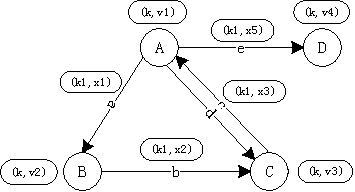
\includegraphics[scale=1.5]{性质图示意图}
\caption{性质图示意图}
\label{性质图示意图}
\end{figure}


\begin{definition}
 \label{性质图定义}
 性质图$G=(V,E,\lambda ,\mu, s,d)$是一个有向的、边标记的、属性化的多重图,$V$是节点的集合,$E$是有向边的集合,$s: E \rightarrow V$和$d:E \rightarrow V$分别是有向边到源节点和目的节点的映射,$\lambda : E \rightarrow \sum $是边标记函数,将一条边映射到字符集$\sum$中的一个字符。节点和边都用键—值对表示性质,性质的赋值函数为$\mu:(V \cup E) \times K \rightarrow S$,$K$和$S$分别是性质的键和值。
\end{definition}

源代码软件漏洞分析依赖于多种代码的中间表示例如语法分析树、抽象语法树、数据流图、控制流图等,对于C/C++,很多编译器的前端能够很容易的通过插桩的方式生成中间表示。但是当分析涉及到复杂的程序或者跨越多个程序搜集中间表示时,编译程序所需要的环境就很难得到保证,特别的是,一般的编译器前端无法处理代码有头文件缺失的情况。与源代码相关的中间表示都直接或者间接的建立在语法分析树的基础上,所以程序性质图的生成首先需要将源代码转换成语法分析树。在语法分析树的基础上生成抽象语法树、控制流图、数据流图,然后将各种中间表示合并为一个统一的表示形式——程序性质图,然后将程序性质图存入图数据库,用查询的方式搜索节点和边。程序性质图的生成过程如图\ref{程序性质图生成过程}所示。

\begin{figure}[htp]
\centering
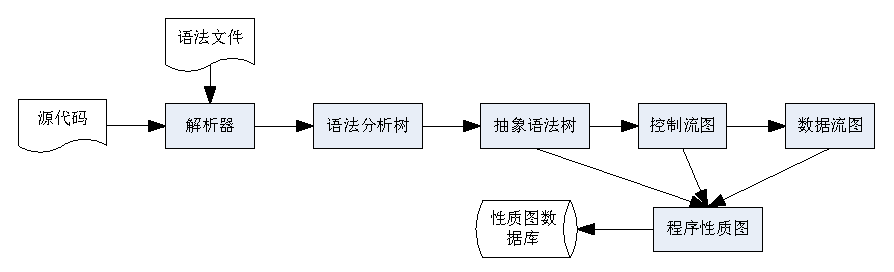
\includegraphics{chap03/程序性质图生成}
\caption{程序性质图生成过程}
\label{程序性质图生成过程}
\end{figure}

\subsection{鲁棒的源代码中间表示生成}
\label{源代码的鲁棒分析}
鲁棒的源代码中间表示生成顺序依次是语法分析树、抽象语法树、控制流图、数据流图。语法分析树建立在ANTLR\upcite{parr_definitive_2013}{(ANother Tool for Language Recognition)}的基础上。ANTLR是一种非常强大的用于读取、执行或者翻译结构性的文本以及二进制文件的解析器生成器,广泛的应用于构建编程语言解析器、工具和框架上。对于C/C++,基于岛屿语法{(Island Grammar)},可以利用ANTLR实现三个层次上的语法解析器:分别是模块解析器、函数解析器以及语句解析器。模块解析器解析粗略的结构信息,例如函数、命名空间以及全局的变量声明。函数解析器解析辨别函数内部能够影响到程序控制流的程序结构,例如跳转语句goto、continue和break;选择语句,如if语句、switch语句;循环语句,如for循环、while循环和do-while循环。语句解析器主要的作用是将任意一个语句分解为表达式、操作符以及标识符等。岛屿语法\upcite{moonen_generating_2001}是一种定义文本结构的语言,通过此语法可以定制解析器的粒度。

图\ref{模块解析器的岛屿语法片段}是模块解析器的岛屿语法片段,第一行中的module表示一个模块,function\_def表示一个函数,simple\_decl表示变量或者类的声明,water表示其他的任意未定义字符,图\ref{模块解析器的岛屿语法片段}表达的意思是一个module可以由一个或者多个functionDef、simple\_decl、using\_directive或者water组成。图\ref{函数解析器的岛屿语法片段}是函数解析器的岛屿语法片段,表示函数有哪些元素组成,其中template\_declStart,return\_type,function\_name,compound\_statement分别表示函数模板、函数返回类型、函数名以及函数内容。图\ref{语句解析器的岛屿语法片段}是语句的岛屿语法片段,第一行表示statements可以由条件编译标识符{(pre\_opener,pre\_closer,pre\_else分别表示\#if,\#endif和\#else)}和语句statement构成。statement的组成当中最主要的是simple\_decl和expr\_statement。expr\_statement是C/C++作为程序主体的每一行代码,在岛屿语法中需要按照运算符的优先级、结合进行设计{(14-17行)}。解析器按照语法文件上规定的顺序解析程序中的非终结符,其他的未被制定的终结符和非终结符用water表示。

\begin{figure}[h]
\begin{lstlisting}[language=C]
module : (function_def | simple_decl | using_directive | water)*;
using_directive: USING NAMESPACE identifier ';';
simple_decl : (TYPEDEF? template_decl_start?) var_decl;
...
water : any_token
\end{lstlisting}
\caption{模块解析器的岛屿语法片段}
\label{模块解析器的岛屿语法片段}
\end{figure}

\begin{figure}[h]
\begin{lstlisting}[language=C]
function_def : template_declStart? return_type? function_name function_paramList ctorList? compound_statement;
template_decl_start : TEMPLATE '<' template_param_list '>';
...
returnType : (functionDeclSpecifiers* typeName) ptrOperator*;
...
function_param_list : '(' parameter_decl_clause? ')' CV_QUALIFIER* exception_specification?;
parameter_decl_clause: (parameter_decl (',' parameter_decl)*) (',' '...')? | VOID;
parameter_decl : param_decl_specifiers parameter_id;
...
function_name: '(' function_name ')' | identifier | OPERATOR operator;
...
compound_statement: opening_curly (statements) closing_curly;
...
\end{lstlisting}
\caption{函数解析器的岛屿语法片段}
\label{函数解析器的岛屿语法片段}
\end{figure}

\begin{figure}[h]
\begin{lstlisting}[language=C]
statements: (pre_opener | pre_closer | pre_else | statement)*;
statement: opening_curly
         | closing_curly
         | block_starter
         | jump_statement
         | label 
         | simple_decl
         | expr_statement
         | water;
...
expr_statement: expr? ';';
expr: assign_expr (',' expr)?;
assign_expr: conditional_expression (assignment_operator assign_expr)?;
conditional_expression: or_expression
		      | or_expression ('?' expr ':' conditional_expression)
or_expression : and_expression ('||' or_expression)?;
and_expression : inclusive_or_expression ('&&' and_expression)?;
...
\end{lstlisting}
\caption{语句解析器的岛屿语法片段}
\label{语句解析器的岛屿语法片段}
\end{figure}

输入一个程序,解析器根据语法文件辨别每一个终结符和非终结符,将这些标识符连接之后会得到语法分析树。语法分析树能够展示编程语言元素的类别、结构以及相互之间的关系.语法分析树是上述解析器输出的唯一表示形式,它忠实的按照语法文件解释源代码的结构细节,其表现形式较为冗余且对微小改动非常敏感。ANTLR内置了生成语法分析树的功能。以第二章图\ref{一个简单的实例程序}为例,生成的语法分析树如图\ref{抽象语法树示意图}所示。

抽象语法树能够直接从语法分析树生成,与语法分析树相比,抽象语法树删除了对程序没有影响的实现细节,更加注重代码的结构,是一种更为紧致简明的中间表示形式也更加的适合于源代码的分析。图\ref{抽象语法树示意图}是图\ref{一个简单的实例程序}的抽象语法树的示意图。抽象语法树能够松的定位和检测程序中的每一行代码以及每行代码中的变量、变量类型操作符等信息,但却不适用于检测代码的执行顺序,所以需要程序的控制流图来展示程序语句的执行顺序以及控制条件。

在辨别程序跳转关键词的基础上,程序的控制流图可以从抽象语法树直接生成,常见的关键词有$if$,$for$以及$goto$。根据这些信息,可以使用以下两步将抽象语法树转换成控制流图。首先,在过程内顺序连接抽象语法树中的语句节点,定义$if$,$for$以及$while$语句转换为控制流图的方式并在所有的抽象语法树上使用此规则;然后处理$break$,$continue$以及$goto$等跳转语句矫正控制流图。实际上,第二阶段仅仅在控制流图上加入了由跳转语句引入的额外的边。图\ref{控制流图}是图\ref{一个简单的实例程序}的控制流图。

每一个程序语句可以使用(use)或者定义(define)变量。如果语句$s2$使用了$s1$定义的变量$v$,且从$s1$到$s2$存在一条路径上,$v$在这条路径中未被重定义,则称$s2$数据依赖于$s1$。将具有数据依赖关系的程序语句使用数据流边连接起来则形成程序的数据流图。图\ref{程序数据流图}是图\ref{一个简单的实例程序}的控制流图。
%\begin{figure}[htp]
%\centering
%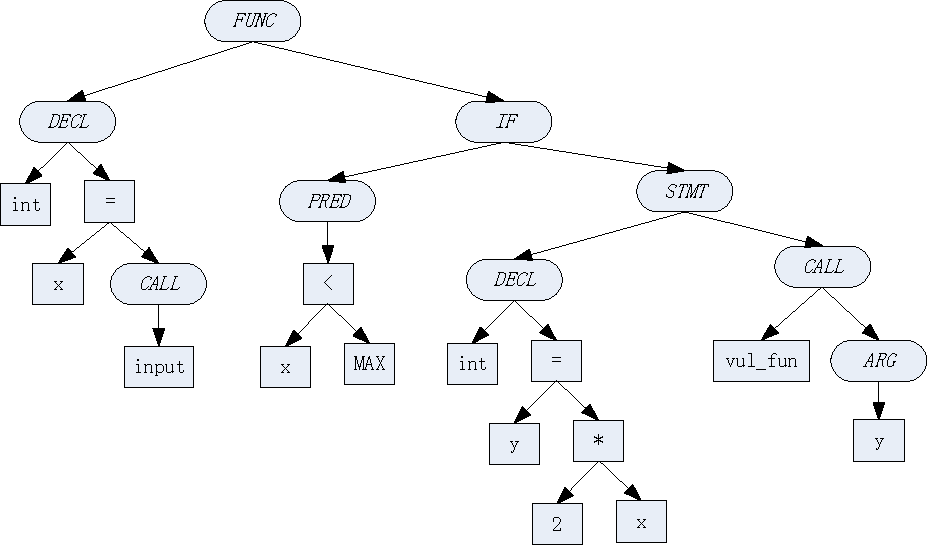
\includegraphics{抽象语法树示意图}
%\caption{Listing \ref{一个简单的实例程序}抽象语法树示意图}
%\label{抽象语法树示意图}
%\end{figure}



%\begin{figure}[htp]
%\centering
%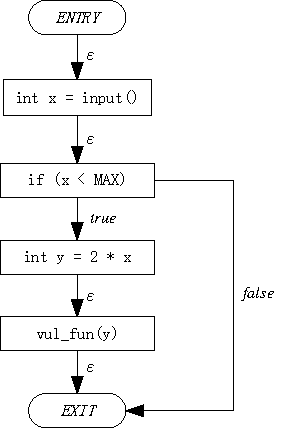
\includegraphics{控制流图}
%\caption{Listing \ref{一个简单的实例程序}控制流图}
%\label{控制流图}
%\end{figure}

%在分析源代码上的漏洞时需要跟踪数据的流向以判断目标语句是否输入可控,这是漏洞是否可利用的一个重要判断依据,与此同时也需要判断目标语句在控制流上是否可达,所以在此引入数据流图。数据流图原本仅仅用于程序切片,现在则成为一个通用的分析数据流以及谓词在程序执行中的作用的工具。数据流图将每个程序语句和谓词都看做一个节点,展示语句和语句之间的数据交互关系。
%\textbf{参考数据依赖和控制依赖的定义来写,不要用那个图}

%\textbf{数据依赖。}程序的每一条语句$s$都会使用{($use$)}或者定义{($define$)}变量。$s$定义了$v$是指$s$将一个值赋给了$v$,这里$s$可以是一个赋值语句也可以是一个输入语句。$s$使用了$v$是指$s$中引用了$v$,例如$v$出现在赋值语句$s$的右半部分,$s$还可以是返回语句、条件语句或者循环语句中的谓词。可以这样定义$use$和$define$操作,$use(s)=\{v | v\text{是}s\text{使用的变量}\}$,$define(s)=\{v | v\text{是}s\text{定义的变量}\}$。语句$s$数据依赖于$use(s)$中的所有变量,定义这些变量的语句和$s$形成数据依赖关系。将所有具有依赖关系的节点连接,则形成数据流图,如图\ref{数据流图}所示。

%\textbf{控制依赖。}一个语句是否能够执行有时会依赖谓词的值,例如Listing \ref{一个简单的实例程序}中vul\_fun(y)执行的条件是谓词x<MAX的值是true。控制依赖关系可以通过控制流图和支配树获取。
%
%Listing \ref{一个简单的实例程序}的控制依赖图如图\ref{数据流图}所示。数据流图打乱了程序节点在控制流图上的顺序,通过给边增加属性值的方式表示数据、控制依赖关系。图中最上层的节点是变量x的定义节点,if语句中的谓词x<MAX使用了变量x并且支配了变量y的定义语句,vul\_fun函数受if语句支配并且使用了变量y。

%\begin{figure}[htp]
%\centering
%\includegraphics{数据流图}
%\caption{Listing \ref{一个简单的实例程序}数据流图}
%\label{数据流图}
%\end{figure}

\subsection{程序性质图}\label{程序性质图}

由于不同种类的源代码软件漏洞具有不同的特征,现存的基于模式匹配的漏洞挖掘工具,一方面不能检测多种源代码软件漏洞,另外一方面则会造成很高的误报,所以需要一种综合的表示形式{——}程序性质图(Code Property Graph, CPG)。
%\upcite{yamaguchi_modeling_2014, yamaguchi_automatic_2015}。
程序性质图可以通过存入专门的图数据库,例如Neo4j\upcite{noauthor_neo4j_nodate},Titan\upcite{noauthor_titan:_nodate}和OrientDB\upcite{noauthor_newsletter_nodate},然后利用数据库查询的方式对程序语句节点以及语句节点之间的关系进行查询。程序性质图是一个抽象语法树性质图、控制流性质图和数据流性质图的综合表示。本节分别定义了三类中间表示的性质图表现形式,然后在此基础上定义程序性质图。

\begin{definition}
\label{抽象语法树定义}
抽象语法树性质图$G _{A}=(V_{A},E_{A},\lambda _{A}, \mu _{A}, s _{A}, d _{A})$,$V_{A}$是抽象语法树节点的集合,$E_{A}$是边集合,$\lambda _{A}$是边的标签函数,用任意字符标记每一条边,$s _{A}$和$d _{A}$是边到节点的映射,分别将边映射到源节点和目的节点。
\end{definition}

抽象语法树节点的性质包括:节点类型{(type)}、代码{(code)}、节点序号{(childnum)}、操作符{(operator)}、位置{(location)、所属文件{(file)}是否控制流节点{(isCFGNode)}。图\ref{抽象语法树性质图实例}为图\ref{一个简单的实例程序}的生成的部分抽象语法树性质图实例。

\begin{figure}[htp]
\centering
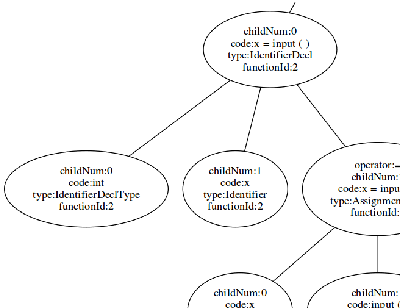
\includegraphics{chap03/抽象语法树性质图实例}
\caption{抽象语法树性质图实例}
\label{抽象语法树性质图实例}
\end{figure}

\begin{definition}
\label{控制流性质图定义}
控制流性质图可以用$G _{C}=(V_{C},E_{C},\lambda _{C}, \mu _{C}, s _{C}, d _{C})$表示,其中$V_{C}=\{ \upsilon | \upsilon \in V_{A} \cup \{ENTRY,EXIT\},\text{且} 对于每一个节点有\mu_C(isCFGNode, type)=True \}$,其中$ENTRY$和$EXIT$是控制流性质图的入口节点和结束节点,$E_{C}$是边的集合,标签函数$\lambda_C$将边映射到字符集 $\sum_C=\{true, false, \epsilon \}$,$true$和$false$用于标记$Condition$语句的两种出边,$\epsilon$用于表示其他没有控制流跳转的边。
\end{definition}

图\ref{控制依赖性质图实例}是图\ref{一个简单的实例程序}的控制依赖性质图的一部分(删除了$ENTRY$节点),从图中可以看出所有节点的$isCFGNode$属性都为$True$。

\begin{figure}[htp]
\centering
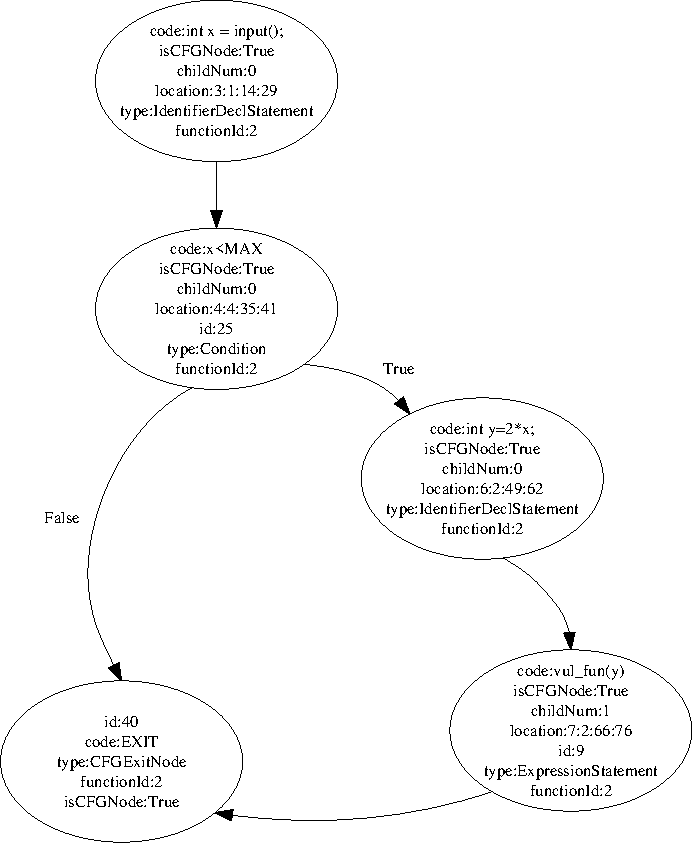
\includegraphics[height=18cm]{chap03/控制依赖性质图实例}
\caption{控制依赖性质图实例}
\label{控制依赖性质图实例}
\end{figure}

\begin{definition}
\label{数据依赖性质图定义}
数据依赖性质图可以用$G _{D}=(V_{D},E_{D},\lambda _{D}, \mu _{D}, s _{D}, d _{D})$表示,其中$V_{D} \subseteq V_C \subseteq V_A$,$E_{D}$是边的集合,标签函数$\lambda_{D} : E_{D} \rightarrow \sum_{D}$,$\sum_{D} = \{D\}$,其中$D$表示数据依赖,同时在表示数据依赖关系的边上增加一个属性$symbol$表示传递的标识符。
\end{definition}

图\ref{数据依赖性质图实例}是图\ref{一个简单的实例程序}的数据依赖图的一部分,此图的节点是是控制流依赖图节点的子集,每条边都有symbol属性表示传递的数据。

\begin{figure}[htp]
\centering
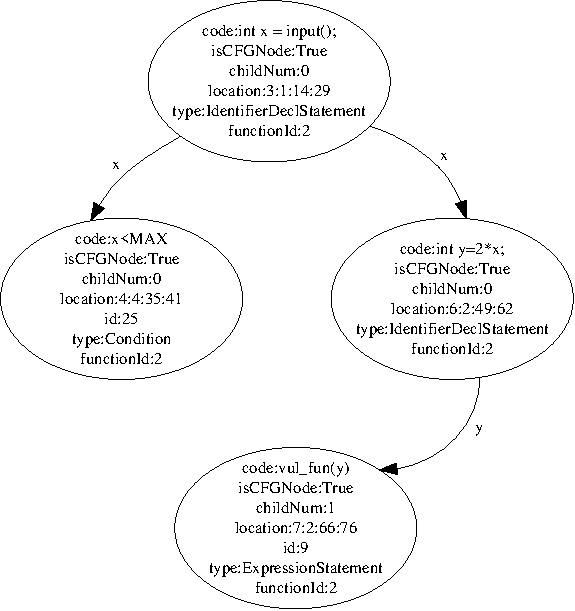
\includegraphics{chap03/数据依赖性质图实例}
\caption{数据依赖性质图实例}
\label{数据依赖性质图实例}
\end{figure}

通过聚合上述三种性质图的定义,可以获得程序性质图的定义如\ref{程序性质图定义}所示。

\begin{definition}
\label{程序性质图定义}
程序性质图可以用$G=(V,E,\lambda, \mu, s, d)$表示,其中$V=V_{A} \cup \{ENTRY, EXIT\}$,$E = E_{A} \cup E_{C} \cup E_{D}$,$\lambda = \lambda_{A} \cup \lambda_{C} \cup \lambda{D} $,$\mu = \mu_{A} \cup \mu_{C} \cup \mu_{D}$,$s = s_{A} \cup s_{C} \cup s_{D}$,$d = d_{A} \cup d_{C} \cup d_{D}$。
\end{definition}

\subsection{程序性质图的基本遍历方式}
\label{程序性质图的基本遍历方式}
生成程序性质图之后,需要有效的数据检索方法用以搜索源代码中特定的代码片段。图数据库提供了专门的查询语言Gremlin\upcite{gremlin},给定节点或边,根据程序性质图边和节点的性质寻找相关节点和边,traversals为其形式化的表现形式。

\begin{definition}
\label{traversal定义}
traversal可以表示为$\tau : P(V \cup E) \rightarrow P(V \cup E)$,其中$V$和$E$分别表示程序性质图的节点和边的集合,$P(V \cup E)$表示$(V \cup E)$的子集。
\end{definition}

最基本的traversal是在性质图数据库中搜索符合条件的节点,称之为过滤器,用$Filter_{p}$表示,如下式所示,其中$p$表示过滤条件的谓词形式。$p$可以任意指定,例如,查找所有$type=Array$的抽象语法树可以表示为$Filter_{\mu(type,Array)}(X)$。
\begin{align*}
Filter_{p} (X) = \{x \in X : p(x) \}
\end{align*}


给定节点搜索查找相应边的traversal可以用下面的公式表示。$X$是所有节点的集合,第一行公式表示在$X$中搜索所有的出边被标记为$l$,且边的性质$k$等于$a$的所有节点。相应的,第二个公式表示在$X$中搜索所有的入边被标记为$l$,且边的性质$k$等于$a$的所有节点。

\begin{align*}
OutE^{k,a}_{l}(X) = \bigcup_{x \in X} \{e: e \in E \ and\ s(e)=x \ and \ \lambda(e) = l \ and \ \mu(e,k) = a \} \\
InE^{k,a}_{l}(X) = \bigcup_{x \in X} \{e: e \in E \ and\ s(e)=x \ and \ \lambda(e) = l \ and \ \mu(e,k) = a \}
\end{align*}

除了根据节点搜索边,根据边查找源节点和目的节点是另外一个基本的traversal,如下式所示。
\begin{align*}
Src(X) = \{s(e): e \in X \} \\
Dst(X) = \{d(e): e \in X \} 
\end{align*}

在搜索具体的代码元素时,需要一些定义一些基本的traversal。给定一个抽象语法树节点,搜索此节点的所有抽象语法子树节点,本章将其定义为$TNode$,如下式所示,其中$Out_{l} (\{v \})$表示查找$\upsilon$的子节点。

\begin{align*}
TNodes(X) = \bigcup_{\upsilon \in X} \big(\upsilon \cup \big( \bigcup_{\upsilon_{c} \in Out_{l} (\{v \}) } TNodes(\{\upsilon_{c} \}) \big) \big)
\end{align*}

给定一个抽象语法树节点,搜索包裹的语句节点也是一个基本需求。例如,已知一个$type=Array$的抽象语法树节点,找到包裹这个节点的语句,然后才能进一步根据语句节点进行控制流分析,其traversal如下式所示。
$$
Statement(X) = \bigcup s(\{ \upsilon \})
$$
$$
\text{其中,}s(X)=\left\{
\begin{aligned}
& X_{1}, & \text{如果} \mu(X_{1}, type)=Stmt \\
& s(In_{l} (X)), & \text{其他}
\end{aligned}
\right.
$$
traversal可以使用复合函数符号$\circ$组合使用。如首先搜索所有的数组节点{($type=Array$的节点)},然后获取这个包裹此节点的语句节点,这个过程可以表示为$Statement \circ Filter_{\mu (\upsilon, type) = Array} (X)$。

\section{基于程序性质图的源代码漏洞挖掘方法研究}\label{基于程序性质图的源代码漏洞粗定位方法研究}
程序性质图里包含了源代码静态分析的所有信息,本小节主要阐述基于程序性质图如何挖掘三种源代码软件漏洞:缓冲区溢出漏洞、格式化字符串漏洞、UAF(Use After Free)漏洞。
%以及Double Free{(DF)}漏洞。

\subsection{缓冲区溢出漏洞挖掘方法研究}
\label{缓冲区溢出漏洞检测}

%\subsubsection{源代码缓冲区溢出漏洞描述}

在程序开发中缓冲区是指在栈或者堆上的一段内存区域,在源代码上表示为一个指向内存的指针或者一个数组变量。在源代码中,缓冲区的写操作有两种形式:(1)内存拷贝函数的调用,如strcpy,strncpy,memcpy,strcat等;(2)数组赋值或者指针解引用赋值;对于内存拷贝函数,如果拷贝的内存大小受输入控制且超过了分配的内存就会造成缓冲区溢出。对于数组赋值或者指针解引用赋值,如果出现在循环内部,在循环控制变量很大或者受输入控制也很容易造成缓冲区溢出。非循环的写操作也可以造成缓冲区溢出,但相对来说溢出的可能性较小。综上,缓冲区溢出漏洞的判定可总结为三个条件:(1)缓冲区的循环写或内存拷贝操作;(2)循环写或内存拷贝操作输入可控;(3)没有边界检测。

内存拷贝函数用MCF{(Memory Copy Functions)}表示,可以分成分两类:第一类包含三个参数,第一个参数是拷贝的目的内存地址,第二个参数是被拷贝的源数据地址,第三个参数是拷贝内存的数量,如strncpy,memcpy等;另外一类包含两个参数,不限制拷贝的内存数量,如strcpy等。对于缓冲区循环写BLW(Buffer Loop Write),在一个函数中判断其是否存在需要两个条件:(1)赋值语句的左半部分是数组索引或者是指针的解引用;(2)赋值语句必须要包含在循环里。对于缓冲区写操作本章统称为BOSink(Buffer Overflow Sinks),所以有$BOSink = MCF \cup BLW$。另外,编程人员自己定义的和内存拷贝函数也需要考虑在内。例如,CVE-2016-9537 \upcite{noauthor_cve_nodate}是一个缓冲区溢出漏洞,溢出的原因是自定义的内存拷贝函数\_TIFFmemcpy没有进行正确的边界检测。此类函数其参数的含义和数量和传统的内存拷贝函数相似,所以这种自定义函数可以和传统的统一进行处理。

输入可控IC(Input Control)是指BOSink中的关键变与和输入变量有数据依赖关系。输入变量可以是函数的参数,也可以通过命令行、环境变量、文件输入或者网络传入的变量。对于包含三个参数的内存拷贝函数如strcnpy,需要满足第二和第三个参数输入可控;对于两个参数的内存拷贝函数如strcpy,需要第二个参数输入可控。内存拷贝函数的输入可控表示为ICMCF(Input Control of Memory Copy Functions)。对于缓冲区的循环写入则要求赋值语句的右操作数、数组索引变量或者循环控制变量输入可控,表示为ICBLW(Input Control of Buffer Loop Write)。所以输入可控可以表示为$IC = ICMCF \cup ICBLW$

缓冲区溢出的边界检测San(Sanitization)包含四种表现形式。

(1)关系表达式中包含内存拷贝函数的长度变量或者表达式,以图\ref{缓冲区溢出边界检测示例代码}中程序为例,
对于第5行的memcpy函数,第4行的边界检测就属于此类,表示为LS(Length Sanitization)。

{(2)}关系表达式中包含内存拷贝函数长度变量所依赖的变量,对于图\ref{缓冲区溢出边界检测示例代码}中第6行的strncpy,表示为LDS(Length Dependency Sanitization)。

(3)关系表达式中包含目的缓冲区变量,对于图\ref{缓冲区溢出边界检测示例代码}中第9行的memcpy函数,第8行的边界检测属于此类,表示为BVS(Buffer Variable Sanitization)。

(4)对于缓冲区循环写,关系表达式中包含循环控制变量,如图\ref{缓冲区溢出边界检测示例代码}中第13行的数组写,第11行的边界检测属于此类,表示为LCVS(Loop Control Variable Sanitization)。

综合以上四种情况,缓冲区溢出边界检测可表示为$San = LS \cup LDS \cup BVS \cup LCVS$。以上四种边界检测判断条件是非常严格的,能够滤除大部分的误报,但同时也一定会引起漏报。

\begin{figure}[h]
\begin{lstlisting}[language=C]
void foo(char *p, int length, int padding)
{
	char dst[255], char dst1[255];
	if(length + padding < 255){
		memcpy(p, dst, length + padding);
		strncpy(dst, p, length);
	}
	if(sizeof(dst) < 255){
		memcpy(p, dst, length);
	}
	if(length<255){
		for(int i=0; i<length; i++){
			dst[i] = 1
		}
	}
}
\end{lstlisting}
\caption{缓冲区溢出边界检测示例代码}
\label{缓冲区溢出边界检测示例代码}
\end{figure}


下面就基于上述的三个条件给出源代码缓冲区溢出的静态模型。
\begin{definition}
\label{缓冲区溢出定义}
缓冲区溢出漏洞可以用一个三元组表示$(IC, BOSink, San)$,其中$IC = ICMCF \cup ICBLW$表示程序的外部输入,$BOSink = MCF \cup BLW$表示缓冲区溢出在源代码上的表示形式,$San = LS \cup LDS \cup BVS \cup LCVS$表示边界检测的四种语法描述。若在一个函数中,某个缓冲区满足$IC$以及$BOSink$,不满足$San$,则表示此函数存在一个缓冲区溢出漏洞。
\end{definition}

%\subsubsection{源代码缓冲区溢出漏洞挖掘算法研究}

程序性质图中承载了所有的检测缓冲区溢出漏洞需要的信息,通过组合不同的traversal可以实现在性质图上检测缓冲区溢出漏洞。内存拷贝函数引起的缓冲区溢出漏洞检测过程如算法\ref{内存拷贝函数缓冲区溢出漏洞检测算法}所示。在检测缓冲器溢出漏洞之前,源代码程序首先被解析并生成程序性质图。算法的输入是一个配置文件,用来记录所要检测的内存拷贝函数名字以及关键的参数次序,返回的是可疑的缓冲区溢出函数已经相应的缓冲区变量,用BOs表示。算法的具体执行过程如下:

%\begin{enumerate}[\textbf{步骤1}]
\begin{enumerate}[(1)]
\item 
从配置文件中导入所要检测的内存拷贝函数名字以及关键的参数次序(第2行);
\item
算法设定两个标识变量flag1和flag2,分别用来判断内存拷贝函数的参数输入可控以及缓冲区无边界检测(第3行);
\item
对于每一个内存拷贝函数获取相应的函数调用AST节点callExpr和对应的参数AST节点args(第5、6行),并且根据args获取语句节点statement,此statement和一样源代码对应,此节点同时也是CFG节点(isCFGNode属性为true);
\item 
对于每一个参数获取参数表达式的符号节点,例如参数是一个表达式a+b,则获取的符号是a和b(第10行);
\item 
判断是否所有的符号都不包含在从输入函数到当前语句的数据流上(第11行),如果判断成立则说明此参数非输入可控,此时flag1设为false(第11-12行);
\item 
根据当前语句节点,沿着控制流图逆向搜索所有的condition节点,对于每一个condition节点,判断是否有symbol是condition的子表达式,如果有说明存在边界检测(第14-17行);
\item 根据flag1和flag2判断内存拷贝函数是否是为缓冲区溢出漏洞,并将当前函数的functionId和location加入到BOs(第21-22行)。
\end{enumerate}

\begin{algorithm}
	\renewcommand{\algorithmicrequire}{\textbf{Input:}}
	\renewcommand{\algorithmicensure}{\textbf{Output:}}
	\caption{内存拷贝函数缓冲区溢出漏洞检测算法}
	\label{内存拷贝函数缓冲区溢出漏洞检测算法}
	\begin{algorithmic}[1]
		\REQUIRE 内存拷贝函数与对应的参数的配置文件 conf
		\ENSURE 缓冲区溢出漏洞可疑函数及缓冲区变量 BOs
		\STATE BOs $\leftarrow \varnothing$
		\STATE MCFAndArgs = loadMCFAndArgs(conf)
		\STATE flag1 $\leftarrow$ true,flag2 $\leftarrow$ true
		\FOR {MCF in MCFAndArgs}
			\STATE MCFCallExprs = findCallASTNode(MCF)
			\FOR{callExpr in MCFCallExprs}
				\STATE statement = findStatementFromChildASTNode(callExpr)
				\STATE args = findKeyArgsFromCallExpr(callExpr)
				\FOR{arg in args}
					\STATE symbols = usedSymbols(arg)
					\IF{ (not DDGEdgeConoveySymbol(symbols)) or not DDGBeginWithInputFunctions(statement))}
						\STATE flag1 = false
					\ENDIF
					\STATE conditions = obtainConditionFromIncomingCFG(statement)
					\FOR{condition in conditions}
						\IF{isInteract(condition, symbols)}
							\STATE flag2 = false
						\ENDIF
					\ENDFOR
				\ENDFOR
				\IF{(flag1 and flag2)}
					\STATE BOs.add(statement.functionId, statement.location)
				\ENDIF
				\STATE flag1 = true, flag2 = true
			\ENDFOR
		\ENDFOR
		
	\STATE return BOs	
	\end{algorithmic}
\end{algorithm}

算法\ref{缓冲区循环写缓冲区溢出漏洞检测算法}是由缓冲区循环写引起的缓冲区溢出漏洞检测过程。此类缓冲区溢出漏洞的检测没有输入,同样输出缓冲区溢出漏洞可疑函数及缓冲区变量,算法的具体执行过程如下:
\begin{enumerate}[(1)]
\item 对于指针解引用造成的缓冲区循环写,首先获取所有的指针解引用AST节点(第2行);
\item 获取指针解引用节点对应的缓冲区变量bufferVar以及此节点对应的语句AST节点statement;
\item 判断当前语句是否是赋值语句,如果是则通过CFG边逆向分析获去控制流节点,判断当前语句节点的控制流是否由循环语句节点流入(第6行);
\item 根据当前语句节点,沿着控制流图逆向搜索所有的condition节点,对于每一个condition节点,判断bufferVar是否为condition的子表达式,如果有说明存在边界检测;
\item 根据flag1和flag2判断指针解引用是否是为缓冲区溢出漏洞(第21-22行),如果flag1和flag2都是true,则将当前的函数和缓冲区变量加入到BOs中;
\item 对于数组赋值形式的缓冲区循环写,首先获取所有的数组索引AST节点arrays(第23行),形如”buf[i]“的都在此列;
\item 对于每一个索引节点,获取当前的语句AST节点statement,继而判断此语句节点是否为赋值语句且是否包含在循环内(第25-26行),如果成立,则获取数组的索引表达式节点indexField(第27行),进而获取indexField使用的所有的符号;例如对于一个在循环内的语句节点"buf[a+b]=1",indexFiled节点为a+b,symbols为[a,b];
\item 对于每一个symbol,判断是否所有的符号都不包含在从输入函数到当前语句的数据流上(第11行),如果成立则说明此参数非输入可控,flag1设为false(第30-31行);
\item 获取数组变量,根据当前语句节点,沿着控制流图逆向搜索所有的condition节点(第34-35行);
\item 沿着控制流图逆向搜索所有的condition节点,对于每一个condition节点,判断bufferVar是否为condition的子表达式或者symbol是否为condition的子表达式,如果有说明存在边界检测,此时设定flag2为false(第36-38行);
\item 根据flag1和flag2判断内存拷贝函数是否是为缓冲区溢出漏洞,并将当前函数的functionId和location加入到BOs(第41-42行)。
\end{enumerate}

\begin{breakablealgorithm}
	\renewcommand{\algorithmicrequire}{\textbf{Input:}}
	\renewcommand{\algorithmicensure}{\textbf{Output:}}
	
	\label{缓冲区循环写缓冲区溢出漏洞检测算法}
	\caption{缓冲区循环写缓冲区溢出漏洞检测算法}
	\begin{algorithmic}[1]
	\REQUIRE 无
	\ENSURE 缓冲区溢出漏洞可疑函数及可疑区域 BOs
	\STATE BOs $\leftarrow \varnothing$
	\STATE dereferences = findDereferenceASTNode()
	\FOR{dereference in dereferences}
		\STATE bufferVar = obtainBufferVar(dereference)
		\STATE statement = findStatementFromChildASTNode(dereference)
		\IF{(isAssignment(statement) and inLoop(statement))}
			\IF{ (\textbf{not} DDGEdgeConoveySymbol(bufferVar)) or (\textbf{not} DDGBeginWithInputFunctions(bufferVar))}
				\STATE flag1 = false
			\ENDIF
			\STATE symbols = usedSymbols(dereference)
			\STATE conditions = obtainConditionFromIncomingCFG(statement)
			\FOR{condition in conditions}
				\IF{isInteract(condition, symbols)}
					\STATE flag2 = false
				\ENDIF
			\ENDFOR
			\IF{(flag1 and flag2)}
				\STATE BOs.add(statement)
			\ENDIF
			\STATE flag1 = true, flag2 = true
		\ENDIF
	\ENDFOR
	\STATE arrays = findArrayASTNode()
	\FOR{array in arrays}
		\STATE statement = findStatementFromChildASTNode(dereference)
		\IF{(isAssig(statement) and inLoop(statement))}
			\STATE indexField = obtainLength(array)
			\STATE symbols = usedSymbols(indexField)
			\FOR{symbol in symbols}
				\IF{ (\textbf{not} DDGEdgeConoveySymbol(symbol)) or (\textbf{not} DDGBeginWithInputFunctions(statement))}
					\STATE flag1 = false
				\ENDIF
			\ENDFOR
			\STATE bufferVar = obtainBufferVar(array)
			\STATE conditions = obtainConditionFromIncomingCFG(statement)
			\FOR{condition in conditions}
				\IF{isInteract(condition, symbols) or isInteract(condition, bufferVar)}
					\STATE flag2 = false
				\ENDIF
			\ENDFOR
			\IF{(flag1 and flag2)}
				\STATE BOs.add(statement.functionId, statement.location)
			\ENDIF
			\STATE flag1 = true, flag2 = true
		\ENDIF
	\ENDFOR
	\STATE return BOs	
	\end{algorithmic}
\end{breakablealgorithm}

\subsection{格式化字符串漏洞挖掘方法研究}
%wb
格式化函数是一系列标准库函数,比如 *printf 系列函数。这些函数接受可变数量的参数,其中一个参数作为其他参数的格式化描述,被称为格式化字符串参数。格式化函数执行时对格式化字符串参数进行解释,并根据其格式描述使用其它的参数填充对应的描述字符串,形成最终的输出。软件编写过程中一般会大量使用这类函数,用于输出、处理字符串等。但是,当格式化字符串与其他输入参数不相符时,就会出现意外情况,比如栈数据泄露,任意内存写等。格式化字符串漏洞一般是指:格式化字符串参数受外部输入影响,从而精心构造的输入可能窃取栈上数据或向内存任意位置写入数据。软件中一般会有很多位置使用格式化函数,如果将他们都直接标记出来,则误报率将会变得相当高,从而导致整个分析过程无效。因此,需要做进一步的分析,尽可能地提高分析精度。
%wb

当调用格式化函数时,格式化字符串参数的来源可分为两种类型:字符串常量类型、变量类型。通过分析漏洞的形成机理和已有的格式化字符串漏洞发现:参数为字符串常量的调用链一般不会出现问题,受输入控制的变量类型则都有可能导致格式化字符串漏洞。输入可控的定义和缓冲区溢出输入可控的定义相同,表示输入函数或者当前函数的参数和格式化函数的参数存在数据依赖关系。基于程序性质图的格式化字符串漏洞的挖掘过程如算法\ref{格式化字符串漏洞检测算法}所示,算法的输出是格式化字符串漏洞可疑函数及可疑区域。格式化字符串漏洞可疑区域是指危险函数中*printf函数调用的行号,此信息由节点的location表示。算法\ref{格式化字符串漏洞检测算法}和算法\ref{内存拷贝函数缓冲区溢出漏洞检测算法}具有很大的相似性。不同的是算法\ref{格式化字符串漏洞检测算法}的输入配置文件是格式化函数和格式化参数的次序组成,例如对于printf函数,其第一个参数是格式化参数,可用一个二元组<printf,0>表示。算法\ref{格式化字符串漏洞检测算法}的具体执行过程如下:
\begin{enumerate}[(1)]
\item 从配置文件导出相应的格式化函数和格式化参数的次序(第2行);
\item 对于每一个格式化函数$fmtFun$,在性质图数据库中搜索所有的名为fmtFun的函数调用AST节点fmtcallExprs,针对每一个fmtcallExpr获取语句节点statement并获取参数节点arg(第3-7行);
\item 
判断arg是否包含在从输入函数到当前语句的数据流上,如果判断成立则将当前函数的functionId和location加入到BOs;
\end{enumerate}

\begin{algorithm}
	\renewcommand{\algorithmicrequire}{\textbf{Input:}}
	\renewcommand{\algorithmicensure}{\textbf{Output:}}
	\caption{格式化字符串漏洞检测算法}
	\label{格式化字符串漏洞检测算法}
	\begin{algorithmic}[1]
		\REQUIRE 格式化函数与对应的参数的配置文件 conf
		\ENSURE 格式化字符串漏洞可疑函数及可疑区域 FSVs
		\STATE FSVs $\leftarrow \varnothing$
		\STATE fmtFunAndArgs = loadFmtFunAndArgs(conf)
		\FOR {fmtFun in FmtFunAndArgs}
			\STATE fmtCallExprs = findCallASTNode(fmtFun)
			\FOR{callExpr in fmtCallExprs}
				\STATE statement = findStatementFromChildASTNode(callExpr)
				\STATE arg = findFmtArgFromCallExpr(callExpr)
				\IF{ (DDGEdgeConoveySymbol(arg)) or DDGBeginWithInputFunctions(statement))}
					\STATE FSVs.add(statement.functionId, statement.location)
				\ENDIF
			\ENDFOR
		\ENDFOR	
	\STATE return FSVs	
	\end{algorithmic}
\end{algorithm}

\subsection{UAF漏洞挖掘方法研究}
%syf
UAF漏洞属于指针相关的漏洞,其主要表现形式是引用已经被释放的内存对象。UAF 漏洞可能导致程序行为异常,经过精心构造的攻击代码可以利用 UAF 漏洞实现任意代码执行。根据 UAF 漏洞的表现形式,可以分析在内存释放函数 (如free、delete 等等) 调用后,被释放的内存对象指针是否任然“存活“,即是否存在后续指令继续使用该指针的行为,如果发现被释放的内存对象指针任然“存活”,则报告一个可疑 UAF 漏洞。要实现上述过程需要分析每一个语句使用的符号和内存释放是否有控制依赖关系,而每个语句节点使用的符号可以由程序符号图PSG(Program Symbol Graph)表示。

\begin{definition}
 \label{符号图定义}
 程序符号图$G_{PS}=(V_{PS},E_{PS},\lambda_{PS} ,\mu_{PS}, s,d)$,$V_{PS}$是所有语句节点和标识符节点$(\mu(type) = identifier)$的集合,$E_{PS}$连接语句节点和语句使用的符号,$\lambda : E \rightarrow \sum_{PS}$是边标记函数,其中$\sum_{PS} = \{use\}$。
\end{definition}

通过将程序符号图引入程序性质图,可以得出基于程序性质图的UAF检测算法,如算法\ref{UAF检测算法}所示。该算法返回的是free函数调用的位置、free的变量再次使用的语句以及当前函数具体的执行过程如下:

\begin{enumerate}[(1)]
\item 初始化返回值以及内存释放函数的名称(第1行),在性质图库中查询所有的内存释放函数的调用语句(第2行);
\item 针对内存释放函数调用语句freeCall,获取所释放内存对应的变量freeVar(第4行),然后在本函数中获取所有控制依赖于freeCall的语句statements(第5行);
\item 对于每一个语句statement,根据符号性质图获取statement使用的所有符号symbols(第7行),判断symbols是否包含freeVar,如果为true说明可能存在一个UAF漏洞,则将freeCall的位置,当前函数Id以及freeVar再次使用的语句位置加入到UAFs中(第9行)。
\end{enumerate}

\begin{algorithm}
	\renewcommand{\algorithmicrequire}{\textbf{Input:}}
	\renewcommand{\algorithmicensure}{\textbf{Output:}}
	\caption{UAF检测算法}
	\label{UAF检测算法}
	\begin{algorithmic}[1]
		\REQUIRE 无
		\ENSURE 内存释放函数调用语句,被free的变量再次使用的语句以及当前函数 UAFs
		\STATE UAFs $\leftarrow \varnothing$,freeCallStr $\leftarrow$\{"free", "delete"\}
		\STATE freeCallExprs = findCallASTNode(freeCallStr)
		\FOR{freeCall in freeCallExprs}
			\STATE freeVar = obtainFreeVar(freeCall)
			\STATE statements = findStatementAlongCFG(freeCall)
			\FOR {statement in statements}
				\STATE symbols = statement.use()
				\IF{symbols.contains(freeVar)}
					\STATE UAFS.add(freeCall.location, statement.location, statement.functionId,)
				\ENDIF
			\ENDFOR
		\ENDFOR
	\STATE return UAFs	
	\end{algorithmic}
\end{algorithm}

%DF(Double Free)漏洞也属于指针相关的漏洞,其主要表现形式是连续释放了同一内存地址。DF漏洞将会破坏程序的内存管理结构,可能导致程序崩溃。同样,经过精心构造的攻击代码可以利用DF漏洞实现任意代码执行。
%DF漏洞的主要特征是两次free操作释放的是同一个内存地址,因此可以通过检测free函数参数是否来自同一定值语句来判断是否存在二次指针释放的可能性。

%\subsection{数据泄露漏洞}

\subsection{实验与分析}

\subsubsection{实验设计}
(1)实验目的

本实验的目的是验证基于程序性质图的源代码软件漏洞挖掘方法在挖掘缓冲区溢出漏洞、格式化字符串漏洞以及UAF漏洞上的有效性。

(2)实验环境与过程

本节在poppler0.10.6、a2ps4.14以及libxml2-2.9.3三个软件上分别对缓冲区溢出漏洞检测算法、格式化字符串漏洞检测算法以及UAF漏洞检测算法进行测试。实验采用的源代码语法解析器ANTLRv4\upcite{parr_definitive_2013},图数据库为Neo4J\upcite{noauthor_neo4j_nodate},图查询语言为Gremlin\upcite{rodriguez_gremlin_2015},漏洞挖掘脚本语言为python。
实验的采用的硬件环境是Inter Xeon CPU E3-1231 v3 @ 3.40GHz,16G RAM。

在漏洞挖掘之前,需要将源代码转化成程序性质图,然后使用算法\ref{内存拷贝函数缓冲区溢出漏洞检测算法}、算法\ref{缓冲区循环写缓冲区溢出漏洞检测算法}挖掘缓冲区溢出漏洞、使用算法\ref{格式化字符串漏洞检测算法}挖掘格式化字符串漏洞、使用算法\ref{UAF检测算法}挖掘UAF漏洞。

\subsubsection{结果分析}

(1)缓冲区溢出漏洞实验

本实验测试的软件是pdf渲染库poppler0.10.6。本实验使用了算法\ref{内存拷贝函数缓冲区溢出漏洞检测算法}与算法\ref{缓冲区循环写缓冲区溢出漏洞检测算法},发现了四个缓冲区溢出漏洞,漏洞对应的文件名,漏洞所在的函数名已经测出的漏洞如表\ref{缓冲区溢出漏洞实验}所示。除了发现的漏洞,本实验还产生了3个误报,误报率为42.9\%。通过调查可知,poppler0.10.6包含11个缓冲区溢出漏洞,漏报率为63.6\%。造成本实验漏报率较高的原因是实际缓冲区溢出漏洞形成原因较为复杂,通过固定的模式很难发现较为复杂的漏洞,因此本章在节\ref{基于机器学习的缓冲区溢出漏洞挖掘方法研究}中提出了一种基于机器学习的缓冲区溢出漏洞挖掘方法,能够以较低的误报率挖掘漏洞。

\begin{table}[ht]
\begin{center}
\caption{缓冲区溢出漏洞实验} \label{缓冲区溢出漏洞实验}
\begin{small}
\begin{tabular}{cccc}
\hline 
文件名 & 函数名 & 是否漏洞 & CVE ID\tabularnewline
\hline 
poppler/Function.cc & PostScriptFunction & N & N/A\tabularnewline
%\rowcolor{gray}
poppler/Function.cc & ExponentialFunction & Y & CVE-2015-8868\tabularnewline

%poppler/Function.cc & SampledFunction & N & N/A\tabularnewline

fofi/FoFiTureType.cc & cvtSfnts & N & N/A\tabularnewline

%\rowcolor{gray}
splash/Splash.cc & transformDataUnit & Y & CVE-2013-1788\tabularnewline

%splash/Splash.cc & clear & N & N/A\tabularnewline
 
%\rowcolor {gray}
fofi/FoFiType1.cc & parse & Y & CVE-2010-3704\tabularnewline

fofi/FoFiType1C.cc & readFDSelect & N & N/A\tabularnewline

%\rowcolor{gray}
splash/Splash.cc & drawImage & Y & CVE-2009-3604\tabularnewline

%splash/SplashXPath.cc & addSegment & N & N/A\tabularnewline
\hline 
\end{tabular}
\end{small}
\end{center}
\end{table}

(2)格式化字符串挖掘实验

本实验用于评估算法\ref{格式化字符串漏洞检测算法},实验的软件是GNU a2ps4.14\upcite{noauthor_a2ps_nodate}。a2ps4.14是一个将各种格式文件转化成PostScript的转换器,支持各种字体且允许用户自定义输出格式。运行算法\ref{格式化字符串漏洞检测算法}输出的结果如表\ref{格式化字符串漏洞实验}所示。算法输出漏洞函数所在文件、函数名以及格式化字符串函数名称。从表中可以看出,本实验在a2ps4.14中发现了一个格式化字符串漏洞。在lib目录下dstring.c文件的第326行,格式化字符串调用语句为vsprintf (ds->content + ds->len, format, args);其格式化字符串参数与函数参数有数据依赖关系,通过查询CVE库发现,其对应的漏洞是CVE-2015-8107。本实验的误报率为87.5\%,但是a2ps4.14中包含484个格式化字符串函数调用,所以总体上本实验大大缩小了需要关注的代码范围。

\begin{table}[ht]
\begin{center}
\caption{格式化字符串漏洞实验} \label{格式化字符串漏洞实验}
\begin{small}
\begin{tabular}{cccc}
\hline 
文件名 & 函数名 & 格式化字符串函数 & 是否漏洞\tabularnewline
\hline 
/lib/printlen.c & printflen & vprintflen & N\tabularnewline
/lib/document.c & documentation\_print\_plain & fprintf & N\tabularnewline
/lib/document.c & documentation\_print\_texinfo & fprintf & N\tabularnewline
/lib/dstring.c & ds\_vsprintf & vsprintf & N\tabularnewline
/lib/dstring.c & ds\_unsafe\_sprintf & ds\_unsafe\_vsprintf & N\tabularnewline
/lib/dstring.c & ds\_cat\_vsprintf & vsprintf & N\tabularnewline
/lib/dstring.c & ds\_unsafe\_vsprintf & vsprintf & N\tabularnewline
%\rowcolor{gray}
/lib/dstring.c & ds\_unsafe\_cat\_vsprintf & vsprintf & Y\tabularnewline
\hline 
\end{tabular}
\end{small}
\end{center}
\end{table}


(3)UAF漏洞挖掘实验

本实验测试的软件是libxml2-2.9.3,libxml2是一个xml c语言版的解析器,本为Gnome项目开发的工具,是一个基于MIT License的免费开源软件。它除了支持c语言版以外,还支持c++、PHP、Pascal、Ruby、Tcl等语言的绑定,能在Windows、Linux、Solaris、MacOsX等平台上运行。表\ref{use after free漏洞挖掘实验}是算法\ref{UAF检测算法}运行在libxml2-2.9.3上的实验结果。算法共检测了2个UAF漏洞对应的CVE编号分别为CVE-2016-1837和CVE-2016-1835。同时也产生了13个误报,误报率为86.7\%。虽然误报率较高,但是libxml2-2.9.3中包含245个内存释放,所以总体上算法\ref{UAF检测算法}大大缩小了需要关注的代码范围。

\begin{table}[ht]
\begin{center}
\caption{Use After Free漏洞挖掘实验} \label{use after free漏洞挖掘实验}
\begin{small}
\begin{tabular}{cccc}
\hline 
文件名 & 函数名 & 是否漏洞 & CVE-ID\tabularnewline
\hline 
tree.c & xmlNodeGetBase & N & N/A\tabularnewline
xmlschemas.c & xmlSchemaGetCanonValueWhtspExt & N & N/A\tabularnewline
HTMLparser.c & htmlParseFile & N & N/A\tabularnewline
HTMLparser.c & htmlFreeParserCtxt & N & N/A\tabularnewline
%\rowcolor{gray}
HTMLparser.c & htmlParseSystemLiteral & Y & CVE-2016-1837\tabularnewline
parse.c & xmlIOParseDTD & N & N/A\tabularnewline
parse.c & xmlNewBlanksWrapperInputStream & N & N/A\tabularnewline
%\rowcolor{gray}
%parse.c & xmlParseNCNameComplex & Y & CVE-2016-1836\tabularnewline
parse.c & xmlParseStartTag2 & Y & CVE-2016-1835\tabularnewline
relaxng.c & xmlRelaxNGNewStates & N & N/A\tabularnewline
relaxng.c & xmlRelaxNGNewValidCtxt & N & N/A\tabularnewline
relaxng.c & xmlRelaxNGValidateDatatype & N & N/A\tabularnewline
relaxng.c & xmlRelaxNGFreeDefine & N & N/A\tabularnewline
relaxng.c & xmlRelaxNGNewDocParserCtxt & N & N/A\tabularnewline
runtest.c & pushParseTest & N & N/A\tabularnewline
xzlib.c & xz\_head & N & N/A\tabularnewline
\hline 
\end{tabular}
\end{small}
\end{center}
\end{table}


\section{基于机器学习的缓冲区溢出漏洞挖掘方法研究}
\label{基于机器学习的缓冲区溢出漏洞挖掘方法研究}

第\ref{缓冲区溢出漏洞检测}节中仅仅考虑了缓冲区写的表现形式和边界检测两个缓冲区溢出的直接因素,同时对缓冲区溢出检测方法执行了非常严格的边界检测策略,即缓冲区大小控制变量不存在任何的条件语句当中,此策略能够非常精确的检测缓冲区溢出漏洞,但同时会造成很多的漏报。在程序的编写过程中,造成缓冲区溢出的因素不仅仅这些,Kratkiewicz\upcite{kratkiewicz_evaluating_2005}将缓冲区溢出漏洞根据不同程序静态特征分成22类。程序静态特征被广泛的应用在建立程序的抽象模型,本小节在程序静态特征的基础上,提出了一种基于机器学习的缓冲区漏洞挖掘方法方法。

%首先,将22种程序静态特征约简成7类,分别是sink类型、缓冲区位置、容器、索引/地址/长度复杂度、边界检测、循环/条件/函数调用深度以及是否输入可控。其次,建立过程间边界检测性质图(ISPG, Inter-procedural Sanitization Property Graph)和函数调用性质图(CCPG, Call Code Property Graph),并将其并入程序性质图,形成扩展程序性质图(ECPG,Extended Property Graph)。然后,在CVE库中查找现存的缓冲区溢出程序和未溢出程序,将此二类分别标记,并利用ECPG获取缓冲区溢出的静态特征并将其映射到向量空间,作为机器学习算法的训练集。最后,选取5种有监督机器学习算法在训练集中训练分类器。5个分类器的平均召回率(recall亦称为TPR,True Positive Rate) 是83.5\%,平均真负率(TNR,True Negative Rate)为85.9\%,最好的召回率达到了96.6\%,最好的真负率达到了91.4\%。因为实验的数据是非均衡数据,所以准确率(Precision)和$F_1$稍低,分别为68.9\%和75.2\%。将此方法应用到poppler0.10.6上,并和经典的静态分析工具FlawFinder做对比,本方法能够将误报率消减到1/12。实验证明,本方法能够有效的辅助挖掘缓冲区溢出漏洞。

\subsection{基本框架}

基于机器学习的缓冲区漏洞挖掘方法的基本思想是通过已存在的漏洞{(本章中如无特别说明,漏洞一词即代表缓冲区溢出漏洞)}去辅助挖掘新的漏洞。本节主要介绍了方法的流程以及各个模块的具体组成和作用。

基于机器学习的缓冲区溢出漏洞挖掘方法的框架包括两个流程相似的过程:训练和分类,如图\ref{fig:基于机器学习的缓冲区溢出漏洞挖掘框架}所示。对于训练流程,首先在CVE漏洞库中手动的查找缓冲区溢出漏洞并标记,通过鲁棒语法分析器对这些代码进行语法分析,然后基于语法分析结果生成扩展的程序性质图并存入性质图数据库,其中扩展程序性质图是将过程间边界检测性质图、函数调用性质图并入程序性质图而形成的;然后利用扩展性质图遍历对程序的缓冲区溢出漏洞静态特征进行提取,最后将提取出来的静态特征向量化并利用多种机器学习算法训练分类器。相似地,对于测试的源代码也需要经历这几个过程,不同的是在提取缓冲区漏洞静态特征并向量化之后,将这些向量数据输入到训练产生的分类器中进行分类,最后生成可疑函数和可疑缓冲区。这里的可疑函数指指被分类器判断包含可疑缓冲区的函数,可疑缓冲区是指可疑函数中代表栈或者堆上的一段内存区域的变量。

\begin{figure}[htp]
\centering
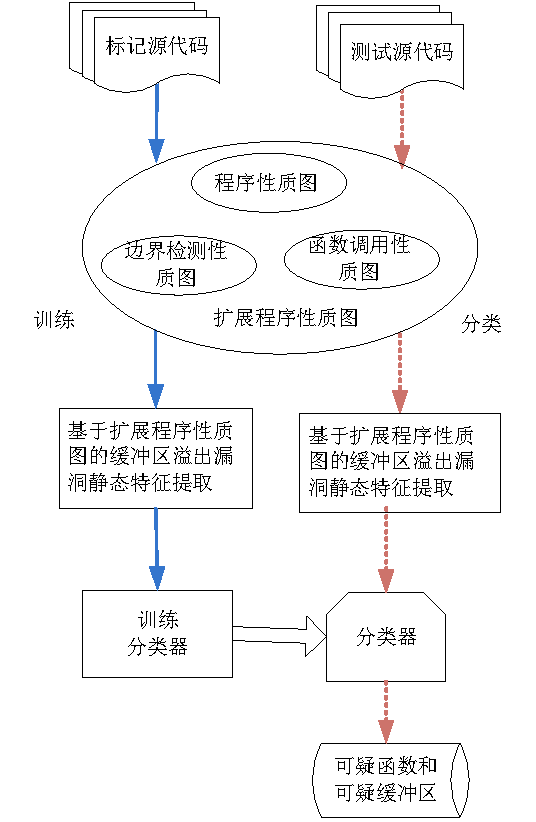
\includegraphics{基于机器学习的缓冲区溢出漏洞挖掘框架}
\caption{基于机器学习的缓冲区溢出漏洞挖掘框架}
\label{fig:基于机器学习的缓冲区溢出漏洞挖掘框架}
\end{figure}

\subsection{程序静态属性与映射规则}

通过分析和总结Kratkiewicz\upcite{kratkiewicz_evaluating_2005}提出的缓冲区溢出漏洞22种分类方法,本小节将缓冲区溢出漏洞的静态属性分为7类,分别为sink类型、缓冲区位置、索引/地址/长度复杂度、边界检测、循环/条件/函数调用深度以及是否输入可控。后续内容详细介绍了各类程序静态属性以及将程序静态属性映射到数字向量空间的规则。

\subsubsection{sink类型}

缓冲区溢出漏洞包含三种sink类型:指针解引用(Pointer Dereference)、数组写(Array Write)以及危险函数(Dangerous Function),如表\ref{Description_of_Three_Sink_Types}所示。如果函数中的一条语句符合三种sink类型的任意一条而又没有进行缓冲区边界检测,则程序就有可能发生缓冲区溢出。在C/C++中,数组的元素即可以通过指针解引用也可以用数组下标访问,但是对同一个缓冲区变量进行访问时很少混合使用,所以这里将二者分成两种类型。例如图\ref{CVE-2016-9537示例代码}中的第24、25行的变量src和dst就属于指针解引用这一类。危险函数是指像memcpy,strncpy等内存函数拷贝、字符串拼接函数,或者用户定义的具有相似功能的函数,例如程序图\ref{CVE-2016-9537示例代码}中第15、16、17行中的用户定义函数“\_TIFFmemcpy”,此函数和标准库函数memcpy的作用相同。如果一个用户定义的函数和标准库函数的参数个数相同、功能相近,则亦将此函数归为危险函数一类。
%另外某些格式化字符串函数也可能引起缓冲区溢出漏洞,但在本节中不予考虑。

\begin{table}[ht]
\begin{center}
\caption{缓冲区溢出漏洞三种sink类型} \label{Description_of_Three_Sink_Types}
\begin{small}
\begin{tabular}{lll}
\hline
{\bf Sink Type} & {\bf Example} & {\bf Mapping Value} \\
\hline
pointer dereference & *p++ = 1 &  1\\
\hline
array write & p[i] = 1 & 2 \\ \hline
dangerous function & strcpy(dst, src), strncpy(dst, src, n)\\
& strcat(dst, src), strncat(dst, src, n) & 3\\
& memcpy(dst, src, n), memmove(dst, src, n) &\\
& gets(str), fgets(str, n, fp)
 &  \\ \hline
\end{tabular}
\end{small}
\end{center}
\end{table}

\begin{figure}[h]
\begin{lstlisting}[language=C]
static int reverseSamplesBytes (uint16 spp, uint16 bps, uint32 width, uint8 *src, uint8 *dst)
  {
   int i;
   uint32  col, bytes_per_pixel, col_offset;
   uint8   bytebuff1;
   unsigned char swapbuff[32];
   if ((src == NULL) || (dst == NULL)){
     TIFFError("reverseSamplesBytes","Invalid input or output buffer");
     return (1);
  }
   bytes_per_pixel  = ((bps * spp) + 7) / 8;
   switch (bps / 8){...
     case 2: for (col = 0; col < (width / 2); col++){
       col_offset = col * bytes_per_pixel;                     
       _TIFFmemcpy (swapbuff, src + col_offset, bytes_per_pixel);
       _TIFFmemcpy (src + col_offset, dst - col_offset - bytes_per_pixel, bytes_per_pixel);
       _TIFFmemcpy (dst - col_offset - bytes_per_pixel, swapbuff, bytes_per_pixel);
     }
    break;
    case 1: /* Use byte copy only for single byte per sample data */
      for (col = 0; col < (width / 2); col++){ 
        for (i = 0; i < spp; i++){
          bytebuff1 = *src;
          *src++ = *(dst - spp + i);
          *(dst - spp + i) = bytebuff1;
        }
        dst -= spp;
      }
 ...}
\end{lstlisting}

\caption{CVE-2016-9537示例代码}
\label{CVE-2016-9537示例代码}
\end{figure}

\subsubsection{缓冲区位置}

缓冲区位置属性(Memory Location)描述的是缓冲区内存分布的位置,即栈、堆、数据段、BSS段与共享内存五种位置。从编程角度上,这五种内存位置的初始化方式是不相同的。局部非静态变量定义在栈上,通过malloc函数动态分配的缓冲区在堆上,数据段上存储的是全局初始化变量,BSS段上存储的是未初始化的全局或者静态变量,共享内存是特别分配的映射进或者映射出程序地址空间,并且通过特殊的操作系统函数(如Linux中的shmget,shmat,shmdt和shmctl)释放的内存区域。本节只考虑栈、堆和数据段三类缓冲区位置。三种内存位置被映射成一个三维向量表示为{(stack,heap,data segment)},提取静态属性时,根据缓冲区的初始化方式进行判断,如果相应的内存位置出现则将其赋为1,否则赋为0。例如图\ref{CVE-2016-9537示例代码}中的指针变量swapbuff,因为被声明为局部变量,所以对应的变量表示为$(1,0,0)$。

\subsubsection{容器}

容器属性(Container)描述的是缓冲区是否包含或者包含在一个什么样的容器当中。一般的,容器结构越复杂缓冲区的使用越容易出现错误。根据Zitser\upcite{zitser_testing_2004}统计,7\%的漏洞缓冲区包含在Union结构中,而在本节的训练集中,近30\%的漏洞包含在不同的容器中,所以这里将容器也作为一个属性,容器属性的示例和映射规则规则如表\ref{Container_Attributes}所示。这里将union和struct二者都映射成2,是因为他们在编程上的相似性,others表示更复杂的结构如多重union或者struct等。


\begin{table}[ht]
\begin{center}
\caption{容器属性} \label{Container_Attributes}
\begin{small}
\begin{tabular}{lll}
\hline
{\bf Instance } & {\bf Container Type} & {\bf Mapping Value} \\
\hline
p[256] & none &  0\\
\hline
p[256][256] & array & 1 \\ \hline
struct.p[256] & struct & 2  \\ 
union.p[256] & union & \\ \hline
ohters & others & 3 \\ \hline
\end{tabular}
\end{small}
\end{center}
\end{table}

\subsubsection{索引/地址/长度复杂度}

索引复杂度属性描述的是数组索引的复杂度,其引入是基于这样一个假设:对于索引值的操作越复杂,数组越容易发生溢出。索引复杂度可以分成六种:常量(constant)、加减法(addition)、乘除法(multiplication)、非线性(non-linear)、函数调用(function call)以及数组访问(array access),如表\ref{Index_Type}所示。加减法操作包括类似加法和减法的操作,自增和自减操作也归入此类。乘除法操作包含乘法、除法以及逐位左移和右移等操作。非线性操作包含取模以及标准库的其他非线性函数例如pow()与sqrt()等。函数调用操作描述的是数组索引操作是否包含函数的返回值(除标准库的非线性函数)。数组访问操作表示数组索引操作是否包含数组访问。尽管很难被利用,常量索引还是有造成缓冲区溢出,所以也被列为索引操作之一。除了常量类型,其他的索引操作类型都有两种不同的呈现方式:p[i-8]和(p-8)[i]。

图\ref{accumulating_the_operations_of_i}是获取复杂度的一个简单的示例。i是数组p的索引变量,沿着数据流获取对i的操作形成一个六维向量{(0,1,0,0,1,1)}。

\begin{table}[ht]
\begin{center}
\caption{索引操作类型} \label{Index_Type}
\begin{small}
\begin{tabular}{lll}
\hline
{\bf Operation Type } & {\bf Instance}\\
\hline
constant & p[256] \\ \hline
addition & p[i+8], p[i-8], (p+8)[i], (p-8)[i] \\ \hline
multiplication & p[i*8], p[i/8], p[i$\gg$8], p[i$\ll$8], (buf+8*n)[i] \\ \hline
non-linear & p[i\%8], p[pow(i, j)], p[sqrt(i)] \\ \hline
function call & p[f(i)], (p+f(n))[i], (getAdtres(n))[i] \\ \hline
array access & p[buf[i]], (p+buf[n])[i], (buf[n])[i] \\ \hline
\end{tabular}
\end{small}
\end{center}
\end{table}

\begin{figure}[htp]
\centering
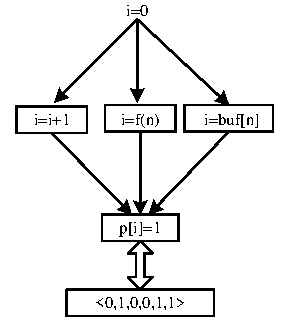
\includegraphics{accumulating_the_operations_of_i}
\caption{变量i复杂度的获取}
\label{accumulating_the_operations_of_i}
\end{figure}

地址/长度复杂度属性与索引复杂度相似,其示例和映射规则如表\ref{ADDRESS_TYPE}和表\ref{LENGTH_TYPE}所示。地址和长度复杂度也被映射成一个六维向量,相应的操作每出现一次对应的值就加1。对于图\ref{CVE-2016-9537示例代码}第24行、25行的缓冲区变量src和dst,地址复杂度属性对应的向量为{(0,1,0,0,0,0)}和{(0,3,0,0,0,0)}。对于危险函数sink类型的缓冲区变量swapbuff,其长度复杂度向量为{(0,1,2,0,0,0)}。另外,索引/地址/长度复杂度属性都需要将缓冲区别名考虑在内,即对缓冲区别名的操作需要类累加到相应的向量中。

\begin{table}[ht]
\begin{center}
\caption{地址操作类型} \label{ADDRESS_TYPE}
\begin{small}
\begin{tabular}{lll}
\hline
{\bf Operation Type } & {\bf Instance}\\
\hline
constant & not appliable \\ \hline
addition & *p(i+8), *p(i-8) \\ \hline
multiplication & *(p+i*8), *p(i/8), *p(i$>>$8), *p(i$<<8$) \\ \hline
non-linear & *(p+i\%8), (p+pow(i, j)), *(p+sqrt(i)) \\ \hline
function call & *(p+f(i)), *(getAddress()) \\ \hline
array access & *(p+buf[i]) \\ \hline
\end{tabular}
\end{small}
\end{center}
\end{table}


\begin{table}[ht]
\begin{center}
\caption{长度操作类型} \label{LENGTH_TYPE}
\begin{small}
\begin{tabular}{lll}
\hline
{\bf Operation Type } & {\bf Instance}\\ \hline
constant & memcpy (dest, src, 256) \\ \hline
addition & memcpy (dest, src, i+256) \\ \hline
multiplication & memcpy (dest, src, i*8) \\ \hline
non-linear & memcpy (dest, src, i\%8) \\ \hline
function call & memcpy (dest, src, f(n)) \\ \hline
array access & memcpy (dest, src, buf[255]) \\ \hline
\end{tabular}
\end{small}
\end{center}
\end{table}

\subsubsection{边界检测}

虽然静态分析不能精确的捕捉缓冲区的边界检测(Sanitization)信息,但依然可以通过边界检测的模式去近似的估计。如果一条语句符合以下的几种模式,就可以近似的认为编程人员已经考虑了边界检测,这些模式出现的次数越多则说明编程人员添加边界检测的概率要更高。边界检测可以分为以下三种类型。

\begin{enumerate}[1]
\item 直接边界检测:假设$P=<n_1, n_2,...,n_N>$是CFG上的一条路径,$0<i<N$。如果$n_j$是一个sink节点,$n_i$是一个条件语句节点,若程序满足以下任一条件,则$n_i$是一个直接边界检测节点。(1)$n_j$是一个数组写sink,$iv$是$n_j$的数组索引变量或表达式,如果$n_i$使用$iv$;(2)$n_j$是一个危险函数sink,$l$是$n_j$索要拷贝的长度变量或者表达式,如果$n_i$使用$l$;(3)$buf$是$n_j$的缓冲区变量且$n_i$使用了$buf$。像$n_i$这样的节点在函数中每出现一次,直接边界检测的值加1。图\ref{CVE-2016-9537补丁程序}第1行的条件语句就是一个直接边界检测。
\item 间接边界检测:此类边界检测只适用于数组写sink和危险函数sink;假设$s$是一个语句节点,$Use(s)=\{v|\text{s是一个定义语句且使用v}\}$,$DDUse(v)$表示所有$v$数据依赖的变量,即$DDUse(v) = \bigcup_{v_c \in Use(v)} v_c \cup DDUse(v_c)$;对于图\ref{CVE-2016-9537示例代码}第15行的长度变量{bytes\_per\_pixel},$DDUse(bytes_per_pixel) = {bps, spp}$;假设$P=<n_1, n_2,...,n_N>$是CFG上的一条路径,$0<i<N$。如果$n_j$是一个sink节点,$n_i$是一个条件语句节点,$iv$是一个长度变量或者数组索引变量,$n_i$使用$v$且$v \in DDUse(iv)$,在$n_i$是一个间接边界检测节点。例如图\ref{间接边界检测示例程序}的第1行就是一个间接边界检测节点。
\item 过程间检测:如果函数的参数与长度变量、数组索引或者缓冲区变量有数据依赖关系,且参数出现在上级调用函数的条件语句中,则称此条件语句是一个过程间边界检测;图\ref{过程间边界检测示例程序}是一个过程间边界检测的示例。
\end{enumerate}

此外,一些条件语句虽然符合上面的描述,但不能算作为边界检测。例如第7行的条件语句不能被当做直接边界检测,因为将一个缓冲区变量和NULL做比较的作用是判断一个指针是否为NULL。边界检测属性被映射成一个三维向量,每一类边界检测出现一次则相应的数值加1。

\begin{figure}[h]
\begin{lstlisting}[language=C]
if( bytes_per_pixel > sizeof(swapbuff) ){
  TIFFError("reverseSamplesBytes","bytes_per_pixel too large");
  return (1);
}

\end{lstlisting}

\caption{CVE-2016-9537补丁程序}
\label{CVE-2016-9537补丁程序}
\end{figure}


\begin{figure}[h]
\begin{lstlisting}[language=C]
if(i<256)
{
  buf[i+j] = 1;
}
\end{lstlisting}

\caption{间接边界检测示例程序}
\label{间接边界检测示例程序}
\end{figure}


\begin{figure}[h]
\begin{lstlisting}[language=C,caption=过程间边界检测示例程序,label=过程间边界检测示例程序]
void woo(int arg){
  if(arg<256)
  {
    foo(arg) ;
  }
}
void foo(int param)
{
  buf[param]=1;
}
\end{lstlisting}

\caption{过程间边界检测示例程序}
\label{过程间边界检测示例程序}
\end{figure}



\subsubsection{循环/条件/函数调用深度}

循环/条件/函数调用深度属性反映了程序的复杂度。其中,循环/条件深度表示包裹sink语句循环/条件层次,函数调用深度描述从入口函数到sink函数之间的函数调用数量,函数调用深度可以通过\ref{扩展的程序性质图}引入的函数调用性质图获取。循环/条件/函数调用深度属性被映射成一个三维向量。对于图\ref{CVE-2016-9537示例代码}的sink变量src,其调用链为$main \rightarrow createCroppedImage \rightarrow mirrorImage \rightarrow reverseSanplesBytes$,switch语句在本节中也被当做条件语句,所以其向量为(2,1,4)。

\subsubsection{输入可控}

输入可控用于判断sink语句是否和输入有数据依赖关系,此属性的判定和\ref{缓冲区溢出漏洞检测}节相同。输入数据可以是函数的参数,也可以通过命令行、环境变量、文件输入或者网络传入的变量。如果sink语句输入可控,则将其设为1,否则设为0。

综上,将七类属性映射的向量串接得到一个18维向量,此向量将被用来训练分类器。

\subsection{扩展的程序性质图}
\label{扩展的程序性质图}

\ref{程序性质图}节中介绍了由过程内的抽象语法树、控制流图以及数据依赖图融合而成的程序性质图。在程序性质图中,每个节点都拥有多个属性,节点之间通过各类边连接,每条边亦拥有多个属性。通过抽象语法树性质图可以获取源代码的所有操作数和操作符,所以sink类型和容器属性可以很容易的获取;获取缓冲区位置和输入可控属性需要抽象语法树和数据依赖图;条件/循环深度需要抽象语法树和控制流图;直接/间接边界检测以及索引/地址/长度复杂度需要三类性质图的结合。但是,程序性质图不能处理过程间边界检测和函数调用深度,因为二者的获取需要过程间的数据依赖和控制依赖关系。为了解决这个问题,将过程间边界检测性质图和函数调用性质图并入到程序性质图形成扩展的程序性质图。

\begin{definition}
 \label{过程间边界检测程序性质图}
 过程间边界检测性质图$G=(V_A,E_{IP},\lambda_{IP} ,\mu_IP, s, d)$,$V_{A}$是抽象语法树节点,$E_{IP}$连接条件语句节点和被调用函数的sink语句节点,$\lambda_{IP}$,$\lambda_{IP}:E_{IP} \rightarrow \sum_{IP}$,其中$\sum_{IP}=\{IC, ID\}$, $IC$表示过程间控制依赖,$ID$表示过程间数据依赖,过程间数据依赖边被赋予一个$symbol$属性。
\end{definition}

图\ref{过程间边界检测和函数调用性质图解释程序}为过程间边界检测和函数调用性质图解释程序。图\ref{简化程序性质图}为其简化的程序性质图(删除了部分抽象语法树节点和边),图\ref{过程间边界检测性质图和函数调用性质图}(a)是的过程间边界检测性质图示意图。通过对比图\ref{简化程序性质图}和图\ref{过程间边界检测性质图和函数调用性质图},可以看出为了产生$E_{IP}$,条件语句if(size<100)必须和函数具有数据和控制依赖关系且memcpy函数的参数src,count必须和foo函数的参数有数据依赖关系。

\begin{definition}
 \label{函数调用性质图}
 过程间边界检测性质图$G=(V_{A},E_{CC},\lambda_{CC} ,\mu_CC, s, d)$,$V_{A}$是抽象语法树节点,如果函数$f_1$调用$f_2$,则$E_{IP}$连接两个函数定义节点,$\lambda_{IP}:E_{CC} \rightarrow \sum_{CC}$,其中$\sum_{IP}=\{CC\}$,每条边被赋予一个$symbol$属性,用于表示函数之间传递的符号。
\end{definition}

图\ref{过程间边界检测性质图和函数调用性质图}(b)图 \ref{过程间边界检测和函数调用性质图解释程序}的函数调用性质图示意图。函数调用性质图能获取函数调用深度,而且能获取影响sink语句的输入源。

\begin{figure}[h]
\begin{lstlisting}[language=C]
int main(int argc, char **argv){
    int i = atoi(argv[1]);
    char *p = argv[2];
    woo(p, i);
}
void woo(char* src, int size){
    if(n<100){
        foo(src, size);
    }
}
void foo(char* src, int n){
    char dst[200];
    int count = n+100;
    memcpy(dst, src, count);
}
\end{lstlisting}

\caption{过程间边界检测和函数调用性质图解释程序}
\label{过程间边界检测和函数调用性质图解释程序}
\end{figure}

\begin{figure}[htp]
\centering
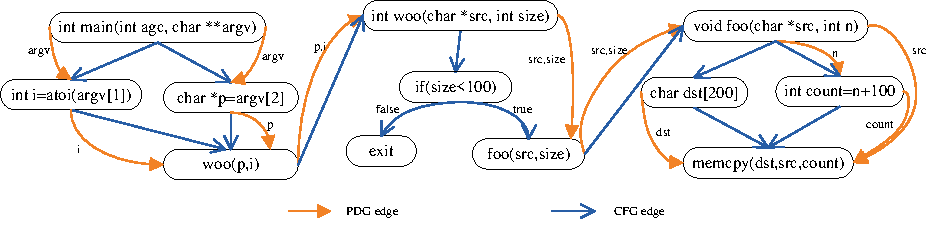
\includegraphics{Simplified_CPG_of_code_for_Fig7}
\caption{图\ref{过程间边界检测和函数调用性质图解释程序}的简化程序性质图}
\label{简化程序性质图}
\end{figure}

\begin{figure}[htp]
\centering
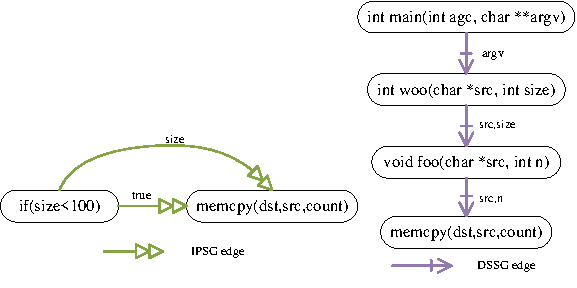
\includegraphics{IPSG_and_DSSG}
\caption{图\ref{过程间边界检测和函数调用性质图解释程序}过程间边界检测性质图和函数调用性质图}
\label{过程间边界检测性质图和函数调用性质图}
\end{figure}

将过程间边界检测性质图,函数调用性质图并入程序性质图形成扩展的程序性质图$G=(V,E,\lambda, \mu, s, d)$,其中,
\begin{align*}
& V = V_{A} \\
& E = E_{A} \cup E_{C} \cup E_{P} \cup E_{IP} \cup E_{CC}\\
& \lambda = \lambda_{A} \cup \lambda_{C} \cup \lambda_{P} \cup \lambda_{IP} \cup \lambda_{CC} \\
& \mu = \mu_{A} \cup \mu_{C} \cup \mu_{P} \cup \mu_{IP} \cup \mu_{CC}
\end{align*}
通过组合程序性质图的基本遍历方式,获取缓冲区溢出漏洞静态属性。

\subsection{实验与分析}

\subsubsection{实验设计}

(1)实验目的与评估参数

通过实验以及和其他工具对比,验证基于机器学习的缓冲区溢出漏洞方法的有效性。方法的性能通过混淆矩阵\upcite{stehman_selecting_1997}展示,如表\ref{confusion_matrix}所示。混淆矩阵描述了实际类别和挖掘类别的交叉组合,即真正类(True Positive,TP),假负类(False Positive,FP),真负类(True Negative,TN)以及假负类(False Negative,FN)。在漏洞挖掘领域,FP又被称为误报,表示一个非漏洞被分类器归为漏洞;FN又称为漏报,表示一个漏洞被分类器归为非漏洞;TP表示一个漏洞被分类器归为漏洞;TN表示一个非漏洞被分类器归为漏洞。在一个正常的程序中,非漏洞函数要远比漏洞函数多,如此会造成训练和测试集的不均衡,所以再次添加了其他的衍生评估参数,即召回率(recall)同时也被称为真值率(True Positive Rate,TPR),真负率(True Negative Rate,TNR),精度(precision)也被称为阳性预测值(Positive Predictive Value,PPV)以及$F_1$值,此四参数的计算如式\ref{衍生标准}所示。

\begin{table}[ht]
\begin{center}
\caption{混淆矩阵} \label{confusion_matrix}
\begin{small}
\begin{tabular}{lll}
\hline
 & {\bf Predicted Positive} & {\bf Actual Positive}\\ \hline
{\bf Actual Positive} & True positive (TP) & False Negative (FN)\\ \hline
{\bf Actual Negative} & False Positive(FP) & True Negative (TN)\\ \hline
\end{tabular}
\end{small}
\end{center}
\end{table}

\begin{equation}
\begin{split}
\label{衍生标准}
& recall = TP/(TP+FN) \\
& TNR = TN/(FP+TN) \\
& precision = TP/(TP+FP) \\
& F_1 = 2 \times (recall \times precision)/(recall + precision)
\end{split}
\end{equation}

(2)实验环境与过程

本方法选取了8个开源软件作为训练集,分别为ffmpeg,HDF5,libtff,mupdf,openssl,qemu,zziplib以及blueZ,如表\ref{CVE_List_For_Attribute_Extraction}所示。从这些软件中,结合CVE漏洞库手动审计了58个缓冲区溢出漏洞函数以及另外的174个非漏洞函数,对于所有的函数,都选择一个缓冲区代表函数提取静态属性。列Vul-Num和Not-Vul-Num分别表示漏洞函数和非漏洞函数数量。漏洞函数被标记为1,非漏洞函数被标记为0。

\begin{table}[ht]
\begin{center}
\caption{实验数据列表} \label{CVE_List_For_Attribute_Extraction}
\begin{small}
\begin{tabular}{llll}
\hline
{\bf Program } & {\bf CVE-ID} & {\bf Vul-Num} & {\bf Not-Vul-Num}\\ \hline
ffmpeg & CVE-2016-7562, CVE-2016-6920, \\ &CVE-2016-10192, CVE-2016-10191,\\ & CVE-2016-10190, CVE-2016-8364,\\ & CVE-2014-5271, CVE-2014-3157,\\ & CVE-2014-2263, CVE-2013-0894,\\ & CVE-2013-0868, CVE-2013-0863,\\ & CVE-2012-0947, CVE-2012-0857,\\ & CVE-2012-0856, CVE-2012-0855,\\ & CVE-2012-0848, CVE-2012-0847 & 18 & 54\\ \hline

HDF5 & CVE-2016-4333, CVE-2016-4330 & 2 & 6 \\ \hline

libtiff & CVE-2017-5225, CVE-2016-9540, \\ & CVE-2016-9537, CVE-2016-9536, \\ & CVE-2016-9535, CVE-2016-9533, \\ & CVE-2016-5652, CVE-2016-5319, \\ & CVE-2016-5318, CVE-2016-5102, \\ & CVE-2016-3991, CVE-2016-3990, \\ & CVE-2016-3632, CVE-2016-3624, \\ & CVE-2015-8784, CVE-2015-8782, \\ & CVE-2013-4244, CVE-2013-4231 & 18 & 54 \\ \hline

mupdf & CVE-2017-5869, CVE-2016-6525, \\ & CVE-2014-2013, CVE-2011-0341 & 4 & 12\\ \hline

openssl & CVE-2016-2182, CVE-2015-0235,\\ & CVE-2014-3512 & 3 & 9\\ \hline

qemu & CVE-2016-7170, CVE-2016-5238,\\ & CVE-2016-4439, CVE-2013-4151,\\ &  CVE-2013-4150 
 & 5 & 15\\ \hline
 
zziplib & CVE-2017-5976, CVE-2017-5975,\\ & CVE-2017-5974, CVE-2017-1614 & 4 & 12\\ \hline

BlueZ & CVE-2016-9917, CVE-2016-9804,\\ & CVE-2016-9803,  CVE-2016-9800 & 4 & 12\\ \hline
\end{tabular}
\end{small}
\end{center}
\end{table}

哪种分类器的性能更好是不可预知的,所以需要测试不同的分类器算法性能。本实验利用了五个著名的分类器:K近邻法(K-Nearest Neighbors,KNN),决策树(Decision Tree,DT),朴素贝叶斯(Naive Bayes,NB),AdaBoost以及支持向量机(Support Vector Machines,SVM)。为了这是的评估分类器性能,本实验采用了10重交叉验证。各分类器参数设定如下:KNN中的参数k为7,DT算法用的是C4.5,AdaBoost使用的弱分类器的数量是20,SVM使用的是RBF核,参数C=10,$\gamma = 0.01$。实验的采用的硬件环境是Inter Xeon CPU E3-1231 v3 @ 3.40GHz,16G RAM。

实验过程如图\ref{fig:基于机器学习的缓冲区溢出漏洞挖掘框架}所示。首先,利用训练集,根据缓冲区溢出漏洞的静态特征训练出分类器;然后,从新的源代码中抽取缓冲区溢出漏洞静态特征并向量化,利用分类器挖掘缓冲区溢出漏洞。

\subsubsection{结果分析}

五个分类器的性能展示如表\ref{PERFORMANCES_OF_OUR_FIVE_CLASSIFIER_ALGORITHMS}所示。平均recall为83.5\%,即58个漏洞平均可以检测出48个。平均TNR是87.3\%,即174个非漏洞152个检测正确。平均precision为68.9\%,平均$F_1$为75.2\%,两个指数不高的原因是训练集是不均衡的,非漏洞是漏洞的3倍。在漏洞检测领域,尽可能的检测最多的漏洞比减少误报更为重要,所以可以认为NB是5个分类器当中表现最好,将96.6\%的漏洞分类正确。

\begin{table}[ht]
\begin{center}
\caption{五个分类器的性能} \label{PERFORMANCES_OF_OUR_FIVE_CLASSIFIER_ALGORITHMS}
\begin{small}
\begin{tabular}{lllllllll}
\hline
 {\bf Classifierss}& {\bf TP} & {\bf FN} & {\bf FP} & {\bf TN} & {\bf recall(\%)} & {\bf TNR(\%)} & {\bf precision(\%)} & {\bf $F_1$(\%)}\\ \hline
KNN & 42 & 16 & 20 & 154 & 72.4 & 88.5 & 67.7 & 70\\ \hline
DT & 44 & 14 & 31 & 143 & 75.9 & 82.2 & 58.7 & 66.2\\ \hline
NB & 56 & 2 & 27 & 147 & 96.6 & 84.5 & 67.5 & 79.5\\ \hline
Adaboosting & 46 & 12 & 15 & 159 & 79.3 & 91.4 & 75.4 & 77.3\\ \hline
SVM & 54 & 4 & 18 & 156 & 93.1 & 89.7 & 75 & 83.1\\ \hline
\end{tabular}
\end{small}
\end{center}
\end{table}

表\ref{PERFORMANCE_OF_BOMINER_FOR_OUR_TEST_SUITE}所示是本章方法和BOMiner\upcite{padmanabhuni_predicting_2014}的对比。
%Padmanabhuni在\upcite{padmanabhuni_predicting_2014}中设计了一个利用机器学习算法挖掘缓冲区溢出漏洞的工具BOMiner。
BOMiner最多能检测出38个漏洞,比本章方法最差的分类器KNN少4个,比最优的分类器NB少18个。BOMiner最高的recall是65.5\%,比本章训练的所有分类器低。图\ref{compareToBOMiner}(a)是本章方法和BOMiner在混淆矩阵平均值上的比较。本章方法平均比BOMiner多发现14.8个漏洞,10.4个非漏洞。图\ref{compareToBOMiner}(b)是本章方法和BOMiner在衍生评估参数平均值上的比较。相比与BOMiner,本章方法在recall上增加了17.5\%,$F_1$值增加了21.1\%。造成性能差距的主要原因是BOMiner并没有更深入的讨论数组写sink和危险函数sink,BOMiner在处理这两类sink时获取的信息太少以至于不能正确的分类漏洞和非漏洞。

\begin{table}[ht]
\begin{center}
\caption{BOMiner性能} \label{PERFORMANCE_OF_BOMINER_FOR_OUR_TEST_SUITE}
\begin{small}
\begin{tabular}{lllllllll}
\hline
 {\bf Classifierss}& {\bf TP} & {\bf FN} & {\bf FP} & {\bf TN} & {\bf TPR(\%)} & {\bf TNR(\%)} & {\bf precision(\%)} & {\bf $F_1$(\%)}\\ \hline
KNN & 29 & 29 & 21 & 153 & 50.0 & 87.9 & 58 & 53.7\\ \hline
DT & 31 & 27 & 35 & 139 & 53.4 & 79.9 & 47 & 50\\ \hline
NB & 38 & 20 & 46 & 128 & 65.5 & 73.6 & 45.2 & 53.5\\ \hline
Adaboosting & 33 & 25 & 28 & 146 & 56.9 & 83.9 & 54.1 & 55.5\\ \hline
SVM & 37 & 21 & 33 & 141 & 63.8 & 81 & 52.9 & 57.8\\ \hline
\end{tabular}
\end{small}
\end{center}
\end{table}

\begin{figure}[htb]
\begin{center}
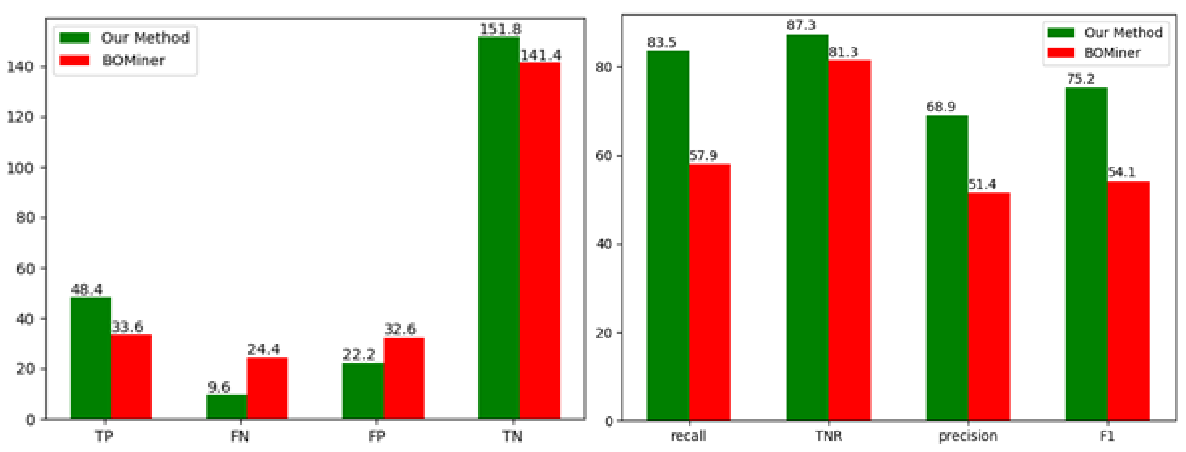
\includegraphics[width=10cm]{compareToBOMiner}
\end{center}
\caption{(a) 和BOMiner在混淆矩阵平均值的比较, (b) 和BOMiner在衍生评估参数上的比较}
\label{compareToBOMiner}
\end{figure}

表\ref{和Joern的混淆矩阵比较}是本章方法和Joern\upcite{yamaguchi_modeling_2014}的性能比较。Joern能够以很低的误报检测源代码缓冲区溢出漏洞。通过设计特定的搜索模式,Joern从linux内核中的驱动中检测了6个缓冲区溢出漏洞。但是,通过研究CVE数据库发驱动中已发现的漏洞有18个,通过分析驱动源代码发现有179个非漏洞sink函数。使用本章方法,最少可以检测12个缓冲区漏洞,五个分类器当中最小的recall是66.7\%,在这两个参数上本章方法要比Joern表现好。最高的TNR是93.8\%,比Joern低6\%。图\ref{compareToJoern}(a)是本章方法在linux驱动上和Joern的比较,本章方法平均比Joern多8.2个漏洞,平均比Joern多11.8个误报。图\ref{compareToJoern}(b)是本章方法衍生参数和Joern的比较,本章方法的平均recall是78.9\%,比Joern高了45.6\%,在TNR上仅仅低了6\%;平均precision比Joern低了24.1\%;平均$F_1$值比Joern高15.5\%。造成性能差异的原因有两个:(1)Joern仅仅专注于memcpy引起的缓冲区漏洞;(2)Joern使用的两个边界检测规则,即目的缓冲区的动态分配和关系表达式都可以当做本章的直接边界检测属性,二者虽然可以减少误报但增加了误报。

\begin{table}[ht]
\begin{center}
\caption{与Joern性能比较} \label{和Joern的混淆矩阵比较}
\begin{small}
\begin{tabular}{lllllllll}
\hline
 {\bf Classifierss}& {\bf TP} & {\bf FN} & {\bf FP} & {\bf TN} & {\bf TPR(\%)} & {\bf TNR(\%)} & {\bf precision(\%)} & {\bf $F_1$(\%)}\\ \hline
Joern & 6 & 12 & 2 & 177 & 33.3 & 98.9 & 75 & 46.2\\ \hline
KNN & 12 & 6 & 11 & 168 & 66.7 & 93.9 & 52.2 & 58.6\\ \hline
DT & 14 & 4 & 14 & 165 & 77.8 & 92.2 & 50 & 60.9\\ \hline
NB & 15 & 3 & 15 & 164 & 83.3 & 91.6 & 50 & 62.5\\ \hline
Adaboosting & 14 & 4 & 12 & 167 & 77.8 & 93.3 & 53.8 & 63.6\\ \hline
SVM & 16 & 2 & 17 & 162 & 88.9 & 90.5 & 48.5 & 62.8\\ \hline
\end{tabular}
\end{small}
\end{center}
\end{table}

\begin{figure}[htb]
\begin{center}
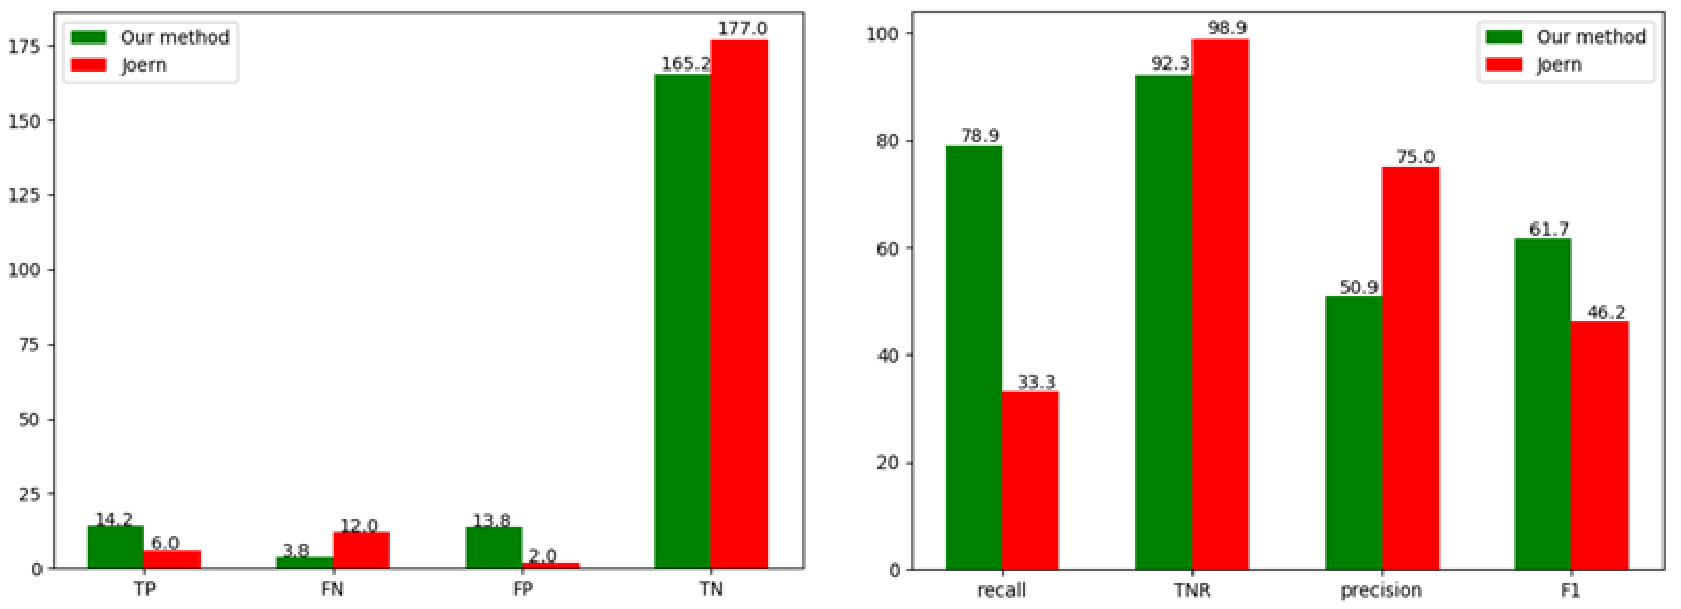
\includegraphics[width=10cm]{compareToJoern}
\end{center}
\caption{(a) 和Joern在混淆矩阵平均值的比较, (b) 和Joern在衍生评估参数上的比较}
\label{compareToJoern}
\end{figure}

除了在在训练集上检验方法的性能,本节在poppler 0.10.6进行了测试,并与FlawFinder做了比较,以验证本章方法在减少可以函数数量的作用。Poppler是一个广泛应用的开源PDF库,历史上被发现了很多漏洞。至今poppler 0.10.6已经被发现了10个被证实的CVE:CVE-2015-8868, CVE-2013-1788, CVE-2010-3704, CVE-2009-3938, CVE-2009-3608, CVE-2009-3607, CVE-2009-3606, CVE-2009-3604以及 CVE-2009-3603。表\ref{PERFORMANCES_OF_OUR_FIVE_CLASSIFIERS_ON_POPPLER0.10.6}展示了5个分类器在poppler 0.10.6的性能,SVFs(Suspect Vulnerable Functions)是TP和FP之和,表示需要考虑的可以函数;Sink (Sink Functions表)示所有的满足三种sink类型的函数;All (All Functions)表示poppler 0.10.6源码中包含的所有函数数量。5个分类器的平均TP为8.8,表示本方法可以检测11个漏洞中的9个。9个CVE有11个漏洞的原因是CVE-2013-1788有三个漏洞函数。平均recall是80\%,平均TNR为94\%,因为非漏洞函数的数量远小于漏洞函数数所以平均$F_1$较低只有28.9\%。从实验结果可以看出,本方法可以以很低的漏报率发现绝大多数漏洞。

Flawfinder\upcite{flawfinder_nodate}是一个基于语法分析的静态漏洞扫描器。当在poppler 0.10.6运行Flawfinder时,其能发现11个中的8个缓冲区溢出漏洞,稍稍低于本章方法。但是Flawfinder同时产生了500误报,是本章方法的12倍之多。以此可以看出,本章方法在缩小可疑函数上效果非常显著。

\begin{table}[ht]
\newcommand{\tabincell}[2]{\begin{tabular}{@{}#1@{}}#2\end{tabular}}
\begin{center}
\caption{五个分类器在Poppler0.10.6上的性能测试} \label{PERFORMANCES_OF_OUR_FIVE_CLASSIFIERS_ON_POPPLER0.10.6}
\begin{small}
\begin{tabular}{llllllllllll}	
\hline
 {\bf }& {\bf TP} & {\bf FN} & {\bf FP} & {\bf TN} & {\bf recall} & {\bf TNR} & {\bf precision} & {\bf $F_1$} & {\bf SVFs} & {\bf Sink} & {\bf All}\\ \hline
KNN & 7 & 4 & 37 & 648 & 63.6 & 94.6 & 15.9 & 25.4 & 44 & \multirowcell{5}{685} & \multirowcell{5}{4876}\\ \cline{1-10}
DT & 8 & 3 & 44 & 641 & 72.7 & 93.6 & 15.4 & 25.4 & 52  \\ \cline{1-10}
NB & 10 & 1 & 52 & 633 & 90.9 & 92.4 & 16.1 & 27.4 & 62  \\ \cline{1-10}
Ada & 9 & 2 & 39 & 646 & 81.8 & 94.3 & 18.8 & 30.6 & 48  \\ \cline{1-10}
SVM & 10 & 1 & 35 & 650 & 90.9 & 94.9 & 22.2 & 35.7 & 45  \\ \hline
\end{tabular}
\end{small}
\end{center}
\end{table}

\section{本章小结}

本章主要研究了基于程序性质图源代码漏洞挖掘方法与基于机器学习的缓冲区溢出漏洞挖掘方法,具体包括以下两个内容。

(1)提出了基于程序性质图的源代码漏洞挖掘方法,用于标定可疑区域。该方法首先利用鲁棒的中间表示生成语法分析树、抽象语法树、控制流图、数据流图;然后通过性质图将三种中间表示聚合成统一的程序性质图,并定义程序性质图遍历方式;最后根据缓冲区溢出漏洞、格式化字符串漏洞以及UAF漏洞的特征给出三类漏洞的挖掘算法。通过在poppler0.10.6、a2ps4.14以及libxml2-2.9.3三个软件上的实验表明,基于程序性质图能够有效的挖掘源代码漏洞。

(2)提出了一种基于机器学习的缓冲区溢出漏洞挖掘方法。该方法首先将22种程序静态特征约简成7类,分别是sink类型、缓冲区位置、容器、索引/地址/长度复杂度、边界检测、循环/条件/函数调用深度以及是否输入可控;其次通过扩展的程序性质图提取静态特征;然后在CVE库中查找现存的缓冲区溢出程序和未溢出程序作为训练集,并选取5种有监督机器学习算法在训练集中训练分类器;最后利用分类器在新的源代码程序中挖掘漏洞。实验结果表明,5个分类器的平均召回率(recall亦称为TPR,True Positive Rate) 是83.5\%,平均真负率(TNR,True Negative Rate)为85.9\%,最好的召回率达到了96.6\%,最好的真负率达到了91.4\%。因为实验的数据是非均衡数据,所以准确率(Precision)和$F_1$稍低,分别为68.9\%和75.2\%。将此方法应用到poppler0.10.6上,并和经典的静态分析工具FlawFinder做对比,本方法能够将误报率消减到1/12。实验证明,本方法能够有效的挖掘缓冲区溢出漏洞。
